\documentclass[10pt,a4paper]{article}

% images
\usepackage[margin=1in]{geometry}
\usepackage{graphicx}
\usepackage{subfig}

% reference items
\usepackage{enumitem}

% links
\usepackage{url}
\usepackage{hyperref}

\usepackage{pdfpages}
\usepackage{pgfplots}

\usepackage{tikz}
\usetikzlibrary{arrows,automata,positioning}

\usepackage{footnote}

% maths
\usepackage{amsmath}
\usepackage{amssymb}
\usepackage{dsfont}
\usepackage{bm}

\usepackage{amsthm}

\theoremstyle{plain}
\newtheorem{theorem}{Theorem}[section]
\newtheorem{claim}[theorem]{Claim}
\newtheorem{lemma}[theorem]{Lemma}

\theoremstyle{definition}
\newtheorem{definition}[theorem]{Definition}

\newenvironment{subproof}[1][\proofname]{%
  \renewcommand{\qedsymbol}{$\blacksquare$}%
  \begin{proof}[#1]%
}{%
  \end{proof}%
}

\newtheorem*{claim*}{Claim}
\newtheorem*{corollary}{Corollary}
\newtheorem*{remark}{Remark}
\newtheorem*{fact}{Fact}

\DeclareMathOperator*{\argmax}{arg\,max}
\DeclareMathOperator*{\argmin}{arg\,min}
 
\newcommand{\code}[1]{\texttt{#1}}
\newcommand*\conj[1]{\overline{#1}}
\newcommand*\vect[1]{\bm{#1}}

% No section numbering
% \setcounter{secnumdepth}{0}

\title{\textbf{Notes on Algorithmic Game Theory}}
\author{Thomas Archbold}
\date{}

\begin{document}
\maketitle

\section{Tragedy of the Commons}
	\begin{itemize}
		\itemsep0em
		\item $n$ players sharing a common resource of limited capacity, normalized e.g. to 1
		\item each player $i$ picks their own level of usage $x_i \in [0,1]$
		\item the quality of the resource deteriorates with increasing usage
	\end{itemize}

	Together the players will pick a vector $\vect{x} = (x_1, \ldots, x_n)
	\in \mathbb{R}^n$, indicating each player's usage.
	Denote total load $\mathcal{L} = \sum_j x_j$, and hence spare capacity = $1
	- \mathcal{L}$. \\

	Denote by $u_i(\vect{x})$ each player's satisfaction/utility of
	their allocation with respect to each other player's use of the resource.
	If the total load is greater than 1, no player gets any satisfaction. Else,
	the satisfaction for player $i$ decreases with increasing total usage, but
	increases with his own usage (up to a point).

	\begin{equation}
		u_i(\vect{x}) = 
		\begin{cases}
			x_i (1 - \mathcal{L}) & \mathcal{L} < 1 \\
			0 & \text{otherwise}
		\end{cases}
	\end{equation}

\subsection{Socially optimal solutions}
	Denote by $u(\vect{x})$ the total satisfaction, i.e. the sum of
	each player's satisfaction according to the allocation vector $\vect{x}$:
	\begin{equation}
		\begin{split}
			u(\vect{x}) & := \sum_j u_j(\vect{x}) \\
				& = \sum_j x_j (1 - \mathcal{L}) \\
				& = (1 - \mathcal{L}) \sum_j x_j \\
				& = (1 - \mathcal{L}) \mathcal{L} \\
				& = \mathcal{L} - \mathcal{L}^2
			\end{split}
			\end{equation}

	Define $u(\mathcal{L}) := \mathcal{L} - \mathcal{L}^2$, i.e. the
	total satisfaction as a function of the total load. \\

	A socially optimal outcome is achieved by maximising this function, so
	$\frac{d}{d\mathcal{L}} u(\mathcal{L}) = -2\mathcal{L} + 1$,
	which is maximised by $\mathcal{L}^* = \frac{1}{2}$. Therefore, a
	benevolent dictator would assign each player an allocation of the shared
	resource such the sum of all the players' allocations is $\frac{1}{2}$.
	Note that the specific allocation to each player doesn't matter, only that
	the total load is $\frac{1}{2}$. \\

	The total satisfaction of this socially optimal solution is
	$u(\mathcal{L}^*) = u(\frac{1}{2}) = \frac{1}{2} -
	(\frac{1}{2})^2 = \frac{1}{4}$. But is this solution stable?

\subsection{The stable solution}
	Self-interest assumption: each player strives to maximise $x_i (1 -
	\mathcal{L})$. With this in mind, define $\mathcal{L}_{-i} := \sum_{j \neq
	i} x_j = (\sum_j x_j) - x_i$. Assuming $\mathcal{L} < 1$, then:
	\begin{equation}
		\begin{split}
			u_i(\vect{x}) & = x_i (1 - \mathcal{L}) \\
			& = x_i (1 - (\mathcal{L}_{-i} + x_i)) \\
			& = x_i (1 - \mathcal{L}_{-i} - x_i)
		\end{split}
	\end{equation}

	Now define $u_i(x_i) := x_i (1 - \mathcal{L}_{-i} - x_i)$.

	\begin{claim}
		$u_i(x_i)$ is maximised by $x_i^* = \frac{1 -
		\mathcal{L}_{-i}}{2}$
	\end{claim}

	\begin{proof}
		$\frac{d}{dx_i} u_i(x_i) = 1 - \mathcal{L}_{-i} - 2x_i$,
		which is maximised at $x_i^* = \frac{1 - \mathcal{L}_{-i}}{2}$
	\end{proof}

	\begin{definition}[Stable solution]
		A solution $\vect{x} = (x_1, \ldots, x_n)$ of the Tragedy of the
		Commons game is stable if no player wants to deviate from it. That is,
		for all $i$, $x_i$ is the best response to $\vect{x}_{-i}$, where
		$\vect{x}_{-i} = (x_1, \ldots, x_{i-1}, x_{i+1}, \ldots, x_n)$.
	\end{definition}

	\begin{claim}
		The \textit{only} stable solution in the Tragedy of the Commons game is
		$\vect{x} = (\frac{1}{n+1}, \ldots, \frac{1}{n+1})$
	\end{claim}

	\begin{proof}
		The solution is stable when no player wishes to deviate. As $u_i(x_i)$
		has one maximum, each player chooses their allocation as $x_i = \frac{1
		- \mathcal{L}_{-i}}{2}$. The total load $\mathcal{L}$ under this
		allocation is:
		\begin{equation*}
			\sum_i x_i = \sum_i \frac{1}{2}(1 - \mathcal{L}_{-i}) = \sum_i
			\frac{1}{2}(1 - (\mathcal{L} - x_i))
		\end{equation*}

		Hence:
		\begin{equation*}
			2 \mathcal{L} = \sum_i 1 - \sum_i \mathcal{L} + \sum_i x_i = n -
			n\mathcal{L} + \mathcal{L}
		\end{equation*}

		So $\mathcal{L} = \frac{n}{n+1} \Rightarrow x_i = \frac{1}{n+1} \text{
			for all } i$.
	\end{proof}

\subsection{The tragedy}
	The total satisfaction of a socially optimal solution $u(\vect{x}^*) =
	\sum_i u_i(\vect{x}^*) = \sum_i x_i (1 - \frac{1}{2}) = \frac{1}{2}
	\sum_i x_i = \frac{1}{4}$.  The spare capacity of the shared resource in
	the stable (self-interested) solution is $1 - \mathcal{L} = 1 -
	\frac{n}{n+1} = \frac{1}{n+1}$, so the total satisfaction in the stable
	solution is:
	\begin{equation}
		\begin{split}
			\sum_i x_i \bigg(\frac{1}{n+1} \bigg) & = \sum_i \frac{1}{n+1} \frac{1}{n+1} \\
			& = \frac{n}{(n+1)^2} < \frac{1}{n}
		\end{split}
	\end{equation}
	
	The tragedy is that not only is the total utility strictly smaller than for
	a socially optimal solution, but it is also bounded by $\frac{1}{n}$,
	meaning the more players there are, the less benefit they get.

\section{Strategic Form Games}

\begin{definition}[Strategic Form Game]
	A \textit{strategic form game} consists of:
	\begin{itemize}
		\itemsep0em
		\item Players ${1, \ldots, n}$
		\item For each player $i$, a finite set $S_i$ of strategies
		\item For each player $i$, the function $u_i : S_1 \times \ldots \times
			S_n \rightarrow \mathbb{R}$ that maps a \textit{strategy profile}
			to a real-numbered payoff to player $i$
	\end{itemize}
\end{definition}

A \textit{strategy profile} is a vector of strategies that fully specifies all
actions in a game. It must include exactly one strategy for each player. Denote
by $\mathcal{S} = \times_i S_i$ the set of all strategy profiles, that is,
$\mathcal{S}$ is the set of all possible combinations of players' strategies.

\begin{remark}
	Each player's utility function is defined as $u_i : \mathcal{S} \rightarrow
	\mathbb{R}$, and not, say, $u_i : S_i \rightarrow \mathbb{R}$.  That is,
	the payoff to player $i$ depends both on his own strategy and the strategy
	chosen by each other player (if the latter were the case, the game would
	only consist of $n$ separate optimization problems, one for each $i$).
\end{remark}

Playing a game consists of:

\begin{enumerate}
	\itemsep0em
	\item simultaneously\footnote{i.e., players do not know what everyone else
		is doing as they are doing it}, each player $i$ chooses a strategy $s_i
		\in S_i$ that strives to maximise their own utility
		(\textbf{self-interest assumption})
	\item each player $i$ receives utility $u_i(s_1, \ldots, s_n)$
\end{enumerate}

\begin{definition}[Strict dominance]
	A strategy $s \in S_i$ \textit{strictly dominates} another strategy $t \in
	S_i$ if for all strategy profiles $s_{-i} \in S_{-i}$:

	\begin{equation}
		u_i(s_{-i}, s) > u_i(s_{-i}, t)
	\end{equation}
\end{definition}

\begin{fact}
	If strategy profiles $s,t \in S_i$ are such that $s$ strictly dominates $t$
	in game $\Gamma$, then the games $\Gamma$ and $\Gamma \setminus t$ are
	equivalent.
\end{fact}

\begin{definition}[Dominance-solvability]
	A game is \textit{dominance solvable} if Iterated Elimination of Strictly
	Dominated Strategies (IESDS) yields a unique strategy profile (i.e. a $1
	\times 1 \times \ldots$ game).
\end{definition}

\begin{fact}
	The outcome of IESDS is always unique, meaning the order of elimination
	does not matter.
\end{fact}

\begin{fact}
	Not all games are dominance-solvable.
\end{fact}

\section{Best responses and Nash Equilibria}

\begin{definition}[Best response]
	A strategy $s^* \in S_i$ is a \textit{best response} of player $i$ to a
	strategy profile $s_{-i}$ if for every other strategy $t \in S_i$:

	\begin{equation}
		u_i(s_{-i}, s^*) \ge u_i(s_{-i}, t)
	\end{equation}
\end{definition}

$s^*$ is therefore the best choice for player $i$ given that the other players
are playing strategies in $s_{-i}$. Player $i$ has no incentive to
\textsc{unilaterally deviate} from $s^*$.

Alternatively and equivalently:

\begin{equation}
	u_i(s_{-i}, s^*) = \max \{ u_i(s_{-i}, t) \, | \, t \in S_i \} = \max_{t \in S_i} u_i(s_{-i}, t)
\end{equation}

\begin{definition}[Pure Strategy Nash Equilibrium]
	A strategy profile $s = (s_1, \ldots, s_n)$ is a Pure Strategy Nash
	Equilibrium (PNE) if for every player $i$, the strategy $s_i$ is a best
	response to $s_{-i}$.
\end{definition}

In other words, in $s = (s_1, \ldots, s_n)$ no player has an incentive to
\textsc{unilaterally deviate}. A PNE is a strategy profile containing only best
responses for each player.

\begin{definition}[Mixed strategy]
	A \textit{mixed strategy} for player $i$ is a probability distribution over
	the set of pure strategies: $\sigma_i = (p(s_1), \ldots, p(s_{|S_i|})) \in
	\Delta^{S_i}$.
\end{definition}

The set of probability distributions $\Delta^{S_i} := \{ (x_1, \ldots,
x_{|S_i|} ) \, : \, \sum_j ^{|S_i|} x_j = 1 \land x_1, \ldots, x_{|S_i|} \ge 0
\}$ defines all probability distributions for player $i$'s strategies. A
probability distribution $\sigma_i$ is a vector detailing the probabilities of
player $i$ choosing each strategy $s \in S_i$, e.g. $\sigma_\text{I} =
(\frac{1}{3}, 0, \frac{2}{3})$.

\begin{definition}[Expected utility]
	Utility functions generalise from pure strategy profiles to mixed strategy
	profiles; the expected utlity for player $i$ under strategy profile $\sigma
	= (\sigma_1, \ldots, \sigma_n)$ is given by:

	\begin{equation}
		\label{eq:expectedUtility}
		u_i(\sigma_1, \ldots, \sigma_n) = \sum_{(S_1, \ldots, S_n) \in
		\mathcal{S}} \prod_j \sigma_j(s_j) \, u_i(s_1, \ldots, s_n)
	\end{equation}
\end{definition}

\begin{definition}[Mixed strategy best response]
	A mixed strategy $\sigma_i$ is a best response of player $i$ to a mixed
	strategy profile $\sigma_{-i}$ if:

	\begin{equation}
		u_i(\sigma_{-i}, \sigma_i) = \max_{\tau \in \Delta^{S_i}} u_i(\sigma_{-i}, \tau)
	\end{equation}
\end{definition}

\begin{definition}[Mixed strategy Nash Equilibrium]
	\label{def:BR}
	Strategy profile $\sigma = (\sigma_1, \ldots, \sigma_n)$ is a \textit{Mixed
	Nash Equilibrium} (MNE) if for every $i$, the strategy $\sigma_i$ is a best
	response to $\sigma_{-i}$.
\end{definition}

Hence in a MNE, no player has an incentive to unilaterally deviate.

\section{Finding Mixed Equilibria in $2\times2$ 2-player games}

Suppose player I and II have two pure strategies $S_\text{I} = \{A, B\}$ and
$S_\text{II} = \{c, d\}$ respectively, and mixed strategies $\sigma_{\text{I}}
= (p, 1-p)$ and $\sigma_{\text{II}} = (q, 1-q)$. That is, for example, player I
plays strategy $A$ with probability $p$ and hence strategy $B$ with probability
$1-p$ (and similarly for player II).  Consider to following payoff matrix:

\begin{center}
	\begin{tabular}{|c|c|c|}
		\hline
		I, II & $c$ & $d$ \\ \hline
		$A$ & 3,1 & 0,0 \\ \hline
		$B$ & 0,0 & 1,3 \\ \hline
	\end{tabular}
\end{center}

To compute the mixed equilibria of this game:

\begin{enumerate}
	\itemsep0em
	\item Draw the diagram of best pure responses of player II to the mixed
		strategy $\sigma_{\text{I}} = (p, 1-p)$ of player I.
	\item Compute $p^* \in [0,1]$ which makes both pure strategies $c$ and $d$
		best responses to $\sigma_{\text{I}}$ \footnote{Equivalently, find the
		mixed strategy $(p^*, 1-p^*)$ which makes player II
		\textit{indifferent} between $c$ and $d$.}.
	\item Repeat for player I
\end{enumerate}

In the above example, playing strategy $c$ player II gets expected payoff that
ranges from 0 (at $p=0$) to 1 (at $p=1$). For strategy $d$ player II's expected
payoff ranges from 3 (at $p=0$) to 0 (at $p=1$).  The resulting lines are shown
in Fig. \ref{fig:expectedUtilityII} -- these are straight lines due to
linearity of expectation.

\begin{center}
	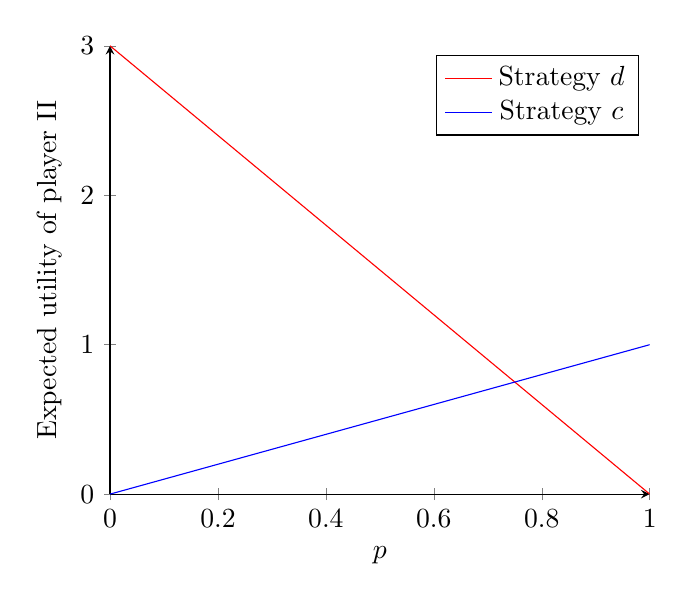
\begin{tikzpicture}
		\label{fig:expectedUtilityII}
		\begin{axis}[
				axis lines = left,
				xlabel = $p$,
				ylabel = {Expected utility of player II},
				]
				\addplot [
					domain=0:1,
					samples=100,
					color=red,
					]{-3*x+3};
					\addlegendentry{Strategy $d$}

					\addplot [
						domain=0:1,
						samples=100,
						color=blue,
						]{x};
						\addlegendentry{Strategy $c$}
		\end{axis}
	\end{tikzpicture}
\end{center}

Think of it this way: if player I plays strategy $A$ with increasing
probability, and player II always plays $c$, player II's utility will increase
from 0 to 1. Similarly, if player I plays strategy $A$ with increasing
probability, and player II always plays $d$, players II's utility will fall
from 3 to 0.

These lines meet at point $p^*$, at which point player II is indifferent to his
choice of strategy (both are best responses).

For step 2, we have:
\begin{equation*}
	\begin{split}
		\mathbb{E}[u_\text{I}((p^*, 1-p^*), c) & =
		\mathbb{E}[u_\text{I}((p^*, 1-p^*), d) \\
		1 p^* + 0 (1 - p^*) & = 0 p^* + 3 (1-p^*) \\
		p^* & = \frac{3}{4}
	\end{split}
\end{equation*}

Repeating for player I, we obtain the following graph:

\begin{center}
	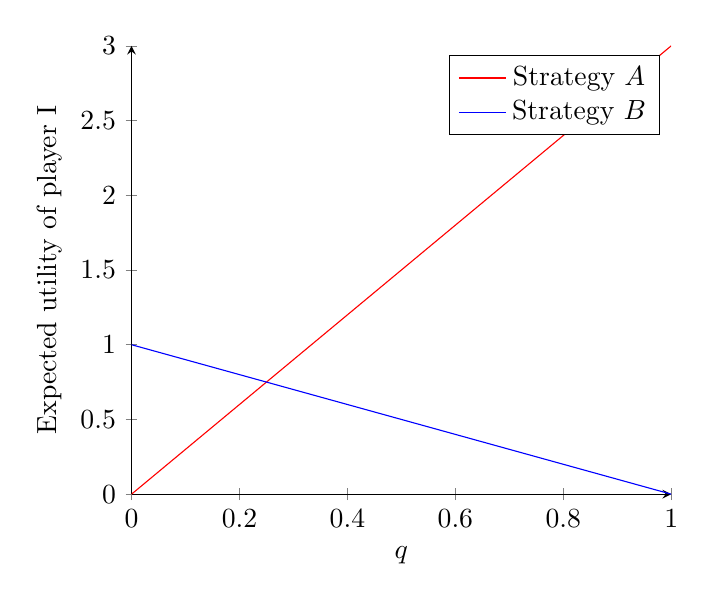
\begin{tikzpicture}
		\label{fig:expectedUtilityI}
		\begin{axis}[
				axis lines = left,
				xlabel = $q$,
				ylabel = {Expected utility of player I},
				]
				\addplot [
					domain=0:1,
					samples=100,
					color=red,
					]{3*x};
					\addlegendentry{Strategy $A$}

					\addplot [
						domain=0:1,
						samples=100,
						color=blue,
						]{-x+1};
						\addlegendentry{Strategy $B$}
		\end{axis}
	\end{tikzpicture}
\end{center}

Again: if player II plays $c$ with increasing probability and I always plays
$A$, I's utility will increase from 0 to 3. If player II plays $c$ with
increasing probability and I always plays $B$, I's utility will decrease from 1
to 0.

These lines meet at $q^*$. Similarly to before, we can compute $q^*$ as before.
Note that:

\begin{equation}
	\begin{split}
		\mathbb{E}[u_\text{I}(A, (q^*, 1-q^*))] & = \mathbb{P}r[A] \mathbb{P}r[c] \, u_\text{I}(A,c) + \mathbb{P}r[A] \mathbb{P}r[d] \, u_\text{I}(A,d) + \mathbb{P}r[B] \mathbb{P}r[c] \, u_\text{I}(B,c) + \mathbb{P}r[B] \mathbb{P}r[d] \, u_\text{I}(B,d) \\
		& = \mathbb{P}r[A] \mathbb{P}r[c] \, u_\text{I}(A,c) + \mathbb{P}r[A] \mathbb{P}r[d] \, u_\text{I}(A,d)
	\end{split}
\end{equation}

The second line comes about as the probability of choosing $B$ in the mixed
strategy $(1, 0)$ is 0, so we can disregard terms involving choosing $B$:

\begin{equation*}
	\begin{split}
		\mathbb{E}[u_\text{I}(A, (q^*, 1-q^*)) & =
		\mathbb{E}[u_\text{I}(B, (q^*, 1-q^*)) \\
		3q^* & = 1 (1-q^*) \\
		q^* & = \frac{1}{4}
	\end{split}
\end{equation*}

Therefore, if such $p^*, q^* \in (0,1)$ exist, then the mixed strategy profile
$((p^*, 1-p^*), (q^*, 1-q^*))$ is a truly mixed-strategy Nash Equilibrium.

\section{Vector-matrix notation for 2-player games}

Let the payoffs to player I be denoted by the matrix $\vect{A}$, where entry
$\vect{A}_{ij}$ gives the payoff to player I when playing strategy $i \in
S_\text{I}$ given that player II is playing strategy $j \in S_\text{II}$.
Define player II's payoff matrix $\vect{B}$ in a similar fashion, where the
rows still represent player I's strategies and the columns player II's.

Let $\vect{x} \in \Delta^{m_1}$ denote player I's mixed strategy, and $\vect{y}
\in \Delta^{m_2}$ denote player II's. Then player I's expected payoff from
playing pure strategy $i \in S_\text{I}$ is given by the entry $(\vect{Ay})_i$,
and player II's expected payoff from playing pure strategy $j \in S_\text{II}$
is given by $(\vect{x^\top B})_j$.

Note when computing player II's expected utility each entry in the resulting
vector is for some fixed column, while when computing player I's then each
entry is for some fixed row.

\subsection{Example}

Suppose we have the following two-player zero-sum (i.e. $\vect{B} = -\vect{A}$)
game:

\begin{equation*}
	\vect{A} = 
	\begin{pmatrix}
		28 & 1 & -38 & -11 \\
		4 & 3 & 2 & -3 \\
		5 & -3 & 4 & 3 \\
		-19 & -9 & 29 & 1
	\end{pmatrix},
	\vect{x} =
	\begin{pmatrix}
		0 \\
		\frac{1}{2} \\
		\frac{1}{2} \\
		0
	\end{pmatrix},
	\vect{y} = 
	\begin{pmatrix}
		0 \\
		\frac{1}{2} \\
		0 \\
		\frac{1}{2}
	\end{pmatrix}
\end{equation*}

In this example, player I's expected utilities $\vect{A} \vect{y} =
\begin{pmatrix} -5 & 0 & 0 & 4 \end{pmatrix}$ and player II's expected
	utilities $\vect{x}^\top \vect{B} = \begin{pmatrix} -\frac{9}{2} & 0 & -3 &
	0 \end{pmatrix}$. Hence pure strategies 2 and 3 are best responses for
	player I to $\vect{y}$ (as they yield the highest expected utility, 0), and
	furthermore player I is indifferent to them. Similarly pure strategies 2
	and 4 are best responses for player II to $\vect{x}$, and is also
	indifferent to them.

Note that:

\begin{equation*}
	\vect{x} =
	\begin{pmatrix}
		0 \\
		\frac{1}{2} \\
		\frac{1}{2} \\
		0
	\end{pmatrix},
	\vect{A} \vect{y} =
	\begin{pmatrix}
		-5 \\
		0 \\
		0 \\
		-4
	\end{pmatrix}
\end{equation*}

Thus $\vect{x}$ is a best response to $\vect{y}$ (strategies 2 and 3 for I are
best responses to $\vect{y}$, and player I mixes between strategies 2 and 3).
Similarly:

\begin{equation*}
	\vect{y} =
	\begin{pmatrix}
		0 \\
		\frac{1}{2} \\
		0 \\
		\frac{1}{2} \\
	\end{pmatrix},
	\vect{x}^\top \vect{B} = 
	\begin{pmatrix}
		-\frac{9}{2} \\
		0 \\
		-3 \\
		0 \\
	\end{pmatrix}
\end{equation*}

Hence $\vect{y}$ is a best response to $\vect{x}$ (strategies 1 and 3 are best
responses, and II mixes between strategies 1 and 3).

\section{Linear Programming and LP Duality}
	A linear program is a linear optimisation problem -- we are maximising
	(minimising) a linear objective function, subject to a set of linear
	constraints (inequalities).

	\begin{definition}[Linear Program]
		Given a matrix $\vect{A} \in \mathbb{R}^{m \times n}$ and vectors
		$\vect{b} \in \mathbb{R}^m, \vect{c} \in \mathbb{R}^n$, we want to
		find a vector $\vect{x} \in \mathbb{R}^n$ such that:
		
		\begin{equation}
			\begin{split}
				\vect{x} \in \argmax \vect{c}^\top \vect{x} \\
				\vect{A}\vect{x} \le \vect{b} \\
				\vect{x} \ge \vect{0}
			\end{split}
		\end{equation}
	\end{definition}

	\subsection{Taking the Dual}
		There are four steps to taking the dual: swap maximise with minimise,
		swap vectors $\vect{b}$ and $\vect{c}$, transpose $\vect{A}$, and
		change the direction of the (non-trivial) inequalities. In the dual
		there is one variable for every constraint, and one constraint for
		every variable. Hence for a primal LP with $n$ variables and $m$
		constraints, the dual LP will have $m$ variables and $n$ constraints.

		Consider the primal linear program, P:
		\begin{equation}
			\begin{split}
				\text{maximise } \vect{c}^\top \vect{x} \text{ subject to }
				\vect{A}\vect{x} & \le \vect{b} \\
				\vect{x} & \ge \vect{0}
			\end{split}
		\end{equation}
	
		The dual of the linear program P, D, is as follows:
		\begin{equation}
			\begin{split}
				\text{minimise } \vect{b}^\top \vect{y} \text{ subject to }
				\vect{A}^\top \vect{y} & \ge \vect{c} \\
				\vect{y} & \ge \vect{0}
			\end{split}
		\end{equation}

		\begin{theorem}[Strong Duality]
			If P or D has an optimal solution of finite value, then so too does
			the other, and the value of the objective function of the optimal
			solutions are equal.
		\end{theorem}

\section{Two-player zero-sum games}

\subsection{Minimax and maximin}

\label{sec:TPZSgames}

Consider a zero-sum game determined by the matrix $\vect{A} \in \mathbb{R}^{m_1
\times m_2}_{\ge 0}$ which gives the payoffs to player I. Since the game is
zero-sum means that the payoff matrix for player II $\vect{B} = -\vect{A}$.

\begin{definition}[Maximin value]
	The maximin value is the highest payoff a player can be sure to receive
	without knowing the actions of the other players. Equivalently, this is the
	lowest value other players can force the player to receive when they know
	the player's action:

	\begin{equation}
		\underline{v_i} = \max_{s_i} \min_{s_{-i}} u_i(s_i, s_{-i})
	\end{equation}
\end{definition}

\begin{definition}[Minimax value]
	The minimax value is the smallest value the other players can force the
	player to receive, without knowing the player's actions. Equivalently, it
	is the largest value the player can be sure to get when they know the
	actions of the other players:

	\begin{equation}
		\overline{v_i} = \min_{s_{-i}} \max_{s_i} u_i(s_i, s_{-i})
	\end{equation}
\end{definition}

Consider the maximin values of the players in a two-player zero-sum game. Since
$u_\text{I}+u_\text{II}=0$, we can denote $u$ as the payoff to player I and
$-u$ as the payoff to player II. Player I's maximin is:
\begin{equation*}
	\underline{v_\text{I}} = \max_{s_\text{I} \in S_\text{I}} \min_{s_\text{II}
	\in S_\text{II}} u(s_\text{I}, s_\text{II})
\end{equation*}

Player II's maximin value is:
\begin{equation*}
		\underline{v_\text{II}} = \max_{s_\text{II} \in S_\text{II}}
		\min_{s_\text{I} \in S_\text{I}} -u(s_\text{I}, s_\text{II}) = -
		\min_{s_\text{II} \in S_\text{II}} \max_{s_\text{I} \in S_\text{I}}
		u(s_\text{I}, s_\text{II})
\end{equation*}

\begin{definition}[Maximin and minimax value in two-player zero-sum games]
	The \emph{maximin value} $\underline{v}$ is the minimum that player I can
	guarantee themselves to get. The \emph{minimax value} $\overline{v}$ is the
	maximum that player II can guarantee they will pay to player I:
	\begin{equation}
		\begin{split}
			\underline{v} & = \max_{s_\text{I} \in S_\text{I}} \min_{s_\text{II}
			\in S_\text{II}} u(s_\text{I}, s_\text{II}) \\
			\overline{v} & = \min_{s_\text{II} \in S_\text{II}} \max_{s_\text{I}
			\in S_\text{I}} u(s_\text{I}, s_\text{II}) \\
		\end{split}
	\end{equation}
\end{definition}

In other words:
\begin{itemize}
	\item maximin value: ``maximum of row minima''
	\item minimax value: ``minimum of column maxima''
\end{itemize}

\textbf{Example}: Consider the following zero-sum game:
\begin{center}
	\begin{tabular}{c|cc}
		& L & R \\ \hline
		T & -2 & 5 \\
		B & 3 & 0 \\
	\end{tabular}
\end{center}

We have:
\begin{equation*}
	\begin{split}
		\underline{v} & = \max \{-2,0\} = 0 \\
		\overline{v} & = \min \{3,5\} = 3
	\end{split}
\end{equation*}

The maximin strategy for player I is the strategy guaranteeing the maximin
value for player I, while the minimax strategy for player II is the strategy
guaranteeing the minimax value for player II. In the above example, player I's
maximin strategy is $B$ and player II's minimax strategy is $L$.

The minimax and maximin values may be equal or, as the example indicates,
different. It must however be the case that $\underline{v} \le \overline{v}$,
since the highest amount that player I can get must be at most the most that
player II will ever pay out to player I.

\begin{fact}
	Maximin value is at most the minimax value: $\underline{v} \le
	\overline{v}$
\end{fact}

\begin{definition}[Value of a game]
	A two-player game has a \emph{value} if $\overline{v}=\underline{v}$. In
	this case the quantity $v:=\overline{v}=\underline{v}$ is called the
	\emph{value of the game}. Any maximin and minimax strategies of player I
	and player II respectively are called \emph{optimal strategies}.
\end{definition}

\begin{definition}[Maximin]
	A strategy $\vect{x}^* \in \Delta^{m_1}$ for player I is a \textit{maximin}
	strategy if

	\begin{equation}
		\vect{x}^* \in \argmax_{\vect{x} \in \Delta^{m_1}} \left[
			\min_{j \in [m_2]} (\vect{x}^\top \vect{A})_j \right]
	\end{equation}
\end{definition}

\begin{definition}[Minimax]
	A strategy $\vect{y}^* \in \Delta^{m_2}$ for player II is a
	\textit{minimax} strategy if

	\begin{equation}
		\vect{y}^* \in \argmin_{\vect{y} \in \Delta^{m_2}} \left[
			\max_{i \in [m_1]} (\vect{A} \vect{y})_i \right]
	\end{equation}
\end{definition}

A maximin strategy ``maximizes the minimum expected payoff to player I''. A
minimax strategy ``minimises the maximum expected payoff to player II''.
Maximin and minimax values can be thought of as \textit{safety utilities} -- no
matter what the other plays, they can set a minimum payoff they will receive.

\begin{itemize}
	\item \textsc{maximin} -- utility that player I can get if he commits to
		move first
	\item \textsc{minimax} -- utility that player II can limit player I's
		utility to if player II commits to move first
\end{itemize}

\begin{theorem}[von Neumann, 1928]
	Let $X \subset \mathbb{R}^n, Y \subset \mathbb{R}^m$ be compact convex
	sets. If $f:X\times Y \rightarrow \mathbb{R}$ is a continuous function that
	is concave-convex, that is:
	\begin{equation*}
		\begin{split}
			& f(\cdot,y): X \rightarrow \mathbb{R} \text{ is concave for fixed } y \\
			& f(x,\cdot): Y \rightarrow \mathbb{R} \text{ is convex for fixed } x \\
		\end{split}
	\end{equation*}

	Then we have that:
	\begin{equation}
		\max_{x \in X} \min_{y \in Y} f(x,y) = \min_{y \in Y} \max_{x \in X}
		f(x,y)
	\end{equation}
\end{theorem}

\subsection{Two-player games as linear programs}

The maximization problem is as follows:

\begin{equation}
	\begin{split}
		\text{maximise}_{\vect{x},v} v \text{ subject to } \vect{x} & \in \Delta^{m_1} \\
		\vect{x}^\top \vect{A} & \ge \begin{pmatrix}
			v \\
			\vdots \\
			v
		\end{pmatrix}
	\end{split}
\end{equation}

Note that this is not yet a Linear Program due to the first constraint. We can
therefore rewrite the optimisation problem as an LP in standard form as:

\begin{equation}
	\begin{split}
		\text{maximise}_{\vect{x},v} v \text{ subject to }
		-\vect{x}^\top \vect{A} + \begin{pmatrix}
			v \\
			\vdots \\
			v
		\end{pmatrix} & \le 0 \\
		\mathds{1}^\top \vect{x} & \le 1 \\
		\vect{x} & \ge 0
	\end{split}
\end{equation}

The primal LP formulation is the following:

\begin{equation}
	\begin{split}
		\text{maximise}_{\vect{x},v}
		(0,\ldots,0,1) \begin{pmatrix}
			x_1 \\
			\vdots \\
			x_{m_1} \\
			v
		\end{pmatrix}
		\text{ subject to }
		\begin{pmatrix}
			& & & 1 \\
			& & & \vdots  \\
			\multicolumn{3}{c}
			{\raisebox{\dimexpr\normalbaselineskip+.7\ht\strutbox-.5\height}[0pt][0pt]
			{{$-\vect{A}^\top$}}} & 1 \\
			1 & \cdots & 1 & 0
		\end{pmatrix} \begin{pmatrix}
			x_1 \\
			\vdots \\
			x_{m_1} \\
			v
		\end{pmatrix} & \le \begin{pmatrix}
			0 \\
			\vdots \\
			0 \\
			1
		\end{pmatrix} \\
		\begin{pmatrix}
			x_1 \\
			\vdots \\
			x_{m_1} \\
			v
		\end{pmatrix} & \ge 0
	\end{split} 
\end{equation}

The dual LP is:

\begin{equation}
	\begin{split}
		\text{minimise}_{\vect{y},w}
		(0,\ldots,0,1) \begin{pmatrix}
			y_1 \\
			\vdots \\
			y_{m_2} \\
			w
		\end{pmatrix}
		\text{ subject to }
		\begin{pmatrix}
			& & & 1 \\
			& & & \vdots  \\
			\multicolumn{3}{c}
			{\raisebox{\dimexpr\normalbaselineskip+.7\ht\strutbox-.5\height}[0pt][0pt]
			{{$-\vect{A}$}}} & 1 \\
			1 & \cdots & 1 & 0
		\end{pmatrix} \begin{pmatrix}
			y_1 \\
			\vdots \\
			y_{m_2} \\
			w
		\end{pmatrix} & \ge \begin{pmatrix}
			0 \\
			\vdots \\
			0 \\
			1
		\end{pmatrix} \\
		\begin{pmatrix}
			y_1 \\
			\vdots \\
			y_{m_2} \\
			w
		\end{pmatrix} & \ge 0
	\end{split} 
\end{equation}

\subsection{LP duality and zero-sum games}

We have the primal (P):

\begin{equation}
	\begin{split}
		\text{max}_{\vect{x}, v} v \text{ subject to }
		\vect{A}^\top \vect{x} & \ge \vect{v} \\
		\mathds{1}^\top \vect{x} & \le 1 \\
		\vect{x} & \ge 0 \\
		\vect{v} & \ge 0
	\end{split}
\end{equation}

We denote by $\vect{v}$ (and analogously for $\vect{w}$) the column vector
$\begin{pmatrix} v \\ \vdots \\ v \end{pmatrix}$. The dual (D) is:

\begin{equation}
	\begin{split}
		\text{min}_{\vect{y}, w} v \text{ subject to }
		\vect{A} \vect{y} & \le \vect{w} \\
		\mathds{1}^\top \vect{y} & \le 1 \\
		\vect{y} & \ge 0 \\
		\vect{w} & \ge 0
	\end{split}
\end{equation}

\begin{fact}
	\label{fact:A}
	For every (P) feasible solution $(\vect{x}, v)$ and for every
	mixed strategy $\vect{y} \in \Delta^{m_2}$, $(\vect{x}^\top
	\vect{A})\vect{y} \ge \vect{v}$.
\end{fact}

This says that the expected utility for player I by playing $\vect{x}$, if
player II chooses any $\vect{y}$, is at least $\vect{v}$.

\begin{proof}
	By the definition of the dot product:
	\begin{equation*}
		\vect{x}^\top \vect{A} \vect{y} = \sum_{j \in [m_2]}
		(\vect{x}^\top \vect{A})_j \cdot \vect{y}_j
	\end{equation*}

	By (P)-feasibility, $\vect{A}^\top \vect{x} \ge 0$ and
	$\vect{y}_j \ge 0$, so:
	\begin{equation*}
		\sum_{j \in [m_2]} (\vect{x}^\top \vect{A})_j \cdot
		\vect{y}_j \ge \sum_{j \in [m_2]} v \cdot \vect{y}_j = v
		\sum_{j \in [m_2]} \vect{y}_j = v
	\end{equation*}
\end{proof}

\begin{fact}
	\label{fact:B}
	If $\vect{A} \ge 0$, then for every (P)-optimal solution $(\vect{x}, v)$ we
	have that $\vect{x} \in \Delta^{m_1}$ is a mixed strategy for player I.
\end{fact}

\begin{proof}
	If $\mathds{1} \vect{x} > 1 - \varepsilon$ for some $\varepsilon > 0$, then
	$(\frac{\vect{x}}{1-\varepsilon}, \frac{v}{1-\varepsilon})$ is also
	(P)-feasible. TODO
\end{proof}

\begin{fact}
	\label{fact:C}
	For every (D)-feasible solution $(\vect{y}, w)$ and for every mixed
	strategy $\vect{x} \in \Delta^{m_1}$, $\vect{x}^\top(\vect{A} \vect{y}) \le
	w$.
\end{fact}

\begin{fact}
	\label{fact:D}
	If $\vect{A} \ge 0$, then for every (D)-optimal solution $(\vect{y}, w)$ we
	have that $\vect{y} \in \Delta^{m_2}$ is a mixed strategy for player II.
\end{fact}

\begin{fact}
	(P) has an optimal solution of finite value.
\end{fact}

\begin{proof}
	The feasible set is non-empty: TODO
\end{proof}

\begin{theorem}[Existence and structure of MNE in zero-sum games]
	For every two-player zero-sum game $\vect{A} \in \mathbb{R}^{m_1 \times
	m_2}_{\ge 0}$, there are mixed strategies $\vect{x} \in \Delta^{m_1},
	\vect{y} \in \Delta^{m_2}$ such that:

	\begin{itemize}
		\item $\vect{x}$ and $\vect{y}$ are maximin and minimax strategies,
			respectively
		\item $(\vect{x}, \vect{y})$ is a Nash Equilibrium
		\item all Nash Equilibria have the same expected payoffs (the
			\textnormal{value} of the game)
	\end{itemize}
\end{theorem}

\begin{proof}
	Let $(x, v)$ and $(y, w)$ be optimal solutions of (P) and (D),
	respectively.

	By the Strong Duality Theorem, we have that $v = w$. Using
	Facts~\ref{fact:A} to \ref{fact:D}, we know that $x$ is a maximin strategy
	for player I, and $y$ is a minimax strategy for player II.

	$x$ and $y$ are mutual best responses, so $(x,y)$ is a Nash Equilibrium.
\end{proof}

\begin{corollary}
	Equilibrium computation in two-player zero-sum games is computable in
	polynomial time.
\end{corollary}

\section{Lemke-Howson Algorithm}

Recall by Definition~\ref{def:BR} that a strategy profile $\sigma^*$ is a MNE
if for every $i$, the strategy $\sigma^*_i$ is a best response to
$\sigma^*_{-i}$ -- that is, for every player $i$ and for every $\sigma_i \in
\Delta^{|S_i|}$ then $u_i(\sigma^*_{-i}, \sigma^*_i) \ge u_i(\sigma^*_{-i},
\sigma_i)$. We have the following lemma:

\begin{lemma}
	Strategy profile $\sigma^*$ is a Mixed Nash Equilibrium iff for each $i$,
	each pure strategy of $i$ is either a best response to $\sigma^*_{-i}$ or
	played with probability 0.
\end{lemma}

The Lemke-Howson algorithm computes Nash Equilibria. We start by drawing the
best response diagrams, yielding polyhedra, then convert these to polytopes by
connecting all lines that go to infinity into a single point.  Then we label
each edge of this polytope with a strategy if that strategy is either a best
response, or if it is played with probability 0. A Nash Equilibrium is
represented by a fully-labelled (i.e. all pure strategies appear as labels)
pair of points in the polytopes. See Fig.~\ref{fig:polytopes} for an example in
a two-player $3\times3$ game.

\begin{figure}[h]
	\centering
	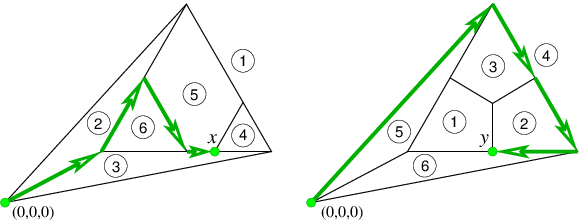
\includegraphics[width=.8\textwidth]{polytopes.png}
	\caption{A run of the Lemke-Howson algorithm}
	\label{fig:polytopes}
\end{figure}

The Lemke-Howson algorithm works by iterating over these two polytopes to find
a pair of fully-labelled vertices. As the number of strategies grows, however,
the number of points on the polytopes grows exponentially.

The procedure is:

\begin{itemize}
	\item Start at a fully-labelled point e.g. $x_1 = \ldots = x_{|S_i|} = 0$.
	\item ``Drop'' a label by traversing an edge in the diagram (this will
		``gain'' another label)
	\item Repeat step 2 until we are at another pair of fully-labelled vertices
\end{itemize}

If the input game is non-degenerate, the the Lemke-Howson algorithm finds at
least one Nash Equilibrium because:

\begin{itemize}
	\item there are finitely many vertices
	\item for a fixed label, the starting edge is unique
	\item for a fixed label, there is a unique continuation from that point
\end{itemize}

Hence we cannot visit any vertex twice.

\subsection{Slack Variables}

We can introduce variables into the constraints to turn the inequalities into
equalities, so that we are only left with non-negativity constraints. Consider
the following game:

\begin{center}
	\begin{tabular}{|c|c|c|}
		\hline
		\textbf{I}, \textbf{II} & 4 & 5 \\ \hline
		1 & 3, 1 & 3, 0 \\ \hline
		2 & 2, 0 & 5, 2 \\ \hline
		3 & 0, 4 & 6, 3 \\ \hline
	\end{tabular}
\end{center}

We get the following polyhedron for player II:

\begin{equation*}
	\begin{split}
		H_\text{II} = \{ (y_4, y_5, v) \, | \, 3y_4 + 3y_5 & \le v \\
		2y_4 + 5y_5 & \le v \\
		6y_5 & \le v \\
		y_4 + y_5 & = 1 \\
		y_4, y_5 & \ge 0 \}
	\end{split}
\end{equation*}

Let's convert this polyhedron to a polytope by dividing each inequality by $v$:

\begin{alignat}{2}
	Q_\text{II} & = \{ y \, | \, \vect{A}y \le 1, y \ge 0 \} \\
	& = \{ (y_4, y_5) \, | \, 3y_4 + 3y_5 & \le 1 \\
	& 2y_4 + 5y_5 & \le 1 \\
	& 6y_5 & \le 1 \\
	& y_4 + y_5 & = 1 \\
	& y_4, y_5 & \ge 0 \}
\end{alignat}

Now introduce new variables $x_1, x_2, x_3$ to turn each inequality into an
equality:

\begin{equation*}
	\begin{split}
		x_1 + 3y_4 + 3y_5 & = 1 \\
		x_2 + 2y_4 + 5y_5 & = 1 \\
		x_3 + 6y_5 & = 1 \\
		x_1, x_2, x_3, y_4, y_5 & \ge 0
	\end{split}
\end{equation*}

These new variables measure the distance of a point within the polytope to the
matching facet\footnote{The facets of an $n$-polytope are the faces of the
polytope with dimension $n-1$. For example, a 3-dimensional cube's facets are
its square faces, but also has 1-dimensional (edges), and 0-dimensional
(points) faces.}. A vertex in the polytope joins two line segments, so
represents two variables being set to 0. Furthermore, variable $i$ is set to 0
if and only if label $i$ is adjacent to the vertex. A solution to a system of
equations is called \textit{basic} if exactly two variables are zero.

\begin{fact}
	Non-degeneracy of a game implies that at most two lines cross at a point.
\end{fact}

\subsection{Dictionary Form}

A system of equations is in \textit{dictionary form} when we express each slack
variable as a function of the original variables. There is exactly one
dictionary per basic solution. In our example, this is:

\begin{equation*}
	\begin{split}
		x_1 & = 1 - 3y_4 - 3y_5 \\
		x_2 & = 1 - 2y_4 - 5y_5 \\
		x_3 & = 1 - 6y_5
	\end{split}
\end{equation*}

\subsection{Pivoting}

Imagine we are increasing the slack variable such that the equality still
holds. This corresponds to dropping that label in the polytope.  We can only
increase the variable so much before some variable on the right hand side (one
of the original variables) becomes 0. In the example above, since $y_4, y_5 \ge
0$, we can see that (ignoring $y_5$) $x_1$ limits $y_4$ to be at most
$\frac{1}{3}$, $x_2$ limits $y_4$ to be at most $\frac{1}{2}$, while $x_3$ does
not limit $y_4$.

\section{Nash's Theorem}
	We prove that every finite game has a Nash Equilibrium by drawing together
	two seemingly unrelated things.

	\subsection{Sperner's Lemma}
	Consider the graph formed from the triangulation of a triangle -- that is,
	a graph that is made up only of smaller triangles.

	\begin{definition}[Valid colouring]
		A valid colouring is a colouring of the vertices, each with a colour in
		the set $\{R,G,B\}$, such that:
		\begin{itemize}
			\item each of the three corners is a distinct colour
			\item no vertex on the side of the big triangle has the same colour
				as the opposite corner
		\end{itemize}
	\end{definition}

	We call a triangle \textit{panchromatic} if each of its vertices have a
	unique colour. We will now state Sperner's Lemma and prove it in two
	different ways.

	\begin{theorem}[Sperner's Lemma]
		Every valid colouring has an odd number of panchromatic triangles.
	\end{theorem}

	\begin{proof}[Proof 1 \emph{(by counting RB triangles)}]
		Let:
		\begin{itemize}
			\item $\bigtriangleup^{RGB} :=$ number of RGB triangles
			\item $\bigtriangleup^{RB} :=$ number of RB triangles
			\item $|^{RB}_X :=$ number of external RB edges, $|^{RB}_I :=$
				number of internal RB edges
		\end{itemize}

		By an external edge, we mean an edge that was formed directly from the
		original triangle, and an internal edge is every edge contained inside
		the triangulation.

		\begin{claim*}
			$|^{RB}_X$ is odd.
		\end{claim*}
		\begin{subproof}
			Consider two corners of the large triangle, where the first is
			coloured red, and the other blue. Since we have a valid colouring,
			no vertex along the edges joining these two corners is coloured
			green, so we only have RB, RR, or BB edges. We get a new RB edge
			whenever we change colour. Since the colours of the corners are
			different, we must change colour an odd number of times, so the
			number of RB edges on the exterior is odd.
		\end{subproof}

		\begin{claim*}
			Each RGB triangle has one RB edge. Each RB triangle has two RB
			edges. All other triangles have 0 RB edges.
		\end{claim*}

		\begin{claim*}
			$\bigtriangleup^{RGB} + 2\bigtriangleup^{RB} = |^{RB}_X +
			2|^{RB}_I$
		\end{claim*}
		\begin{subproof}
			The number of RB edges is equal to
			$\bigtriangleup^{RGB}+2\bigtriangleup^{RB}$. This counts all
			the interior RB edges twice, as each internal edge separates two
			triangles, and each external RB edge once, as exactly one triangle
			touches it.
		\end{subproof}

		Hence $\bigtriangleup^{RGB} = |^{RB}_X + 2|^{RB}_I -
		2\bigtriangleup^{RB} = 2(|^{RB}_I - \bigtriangleup^{RB}) +
		|^{RB}_X$, which is odd.
	\end{proof}

	\begin{proof}[Proof 2 \emph{(by following the End-of-a-Line)}]
		Construct a directed graph based on the triangulation as follows:
		\begin{itemize}
			\item add edges from the B corner to all vertices on the RB side
			\item create a node for each cell (internal triangle), and one for
				the ``outside'' edge
			\item create a directed arc across every RB edge, where R is ``to
				the left'' as we traverse the arc)
		\end{itemize}

		Every node has in-degree at most one and out-degree at most one. Thus
		the graph consists only of isolated vertices, edge-disjoint paths, and
		edge-disjoint cycles. By the Handshaking Lemma, the number of nodes of
		degree exactly one is even. Nodes with degree exactly one appear 
		in panchromatic triangles (one way in, no way out), and only RGB
		triangles contain these nodes of degree exactly one. We began by
		creating an artificial node outside of the large triangle -- every
		other node of degree one corresponds to a panchromatic triangle. Hence
		the number of nodes of degree exactly one in the original graph is odd,
		so the number of RGB triangles in the original graph is odd.
	\end{proof}

	\subsection{Brouwer's Fixed Point Theorem}
	A $k$-simplex is a $k$-dimensional polytope that is the convex hull of its
	$k+1$ vertices. The standard simplex that we will make use of is a simplex
	formed from $k+1$ standard unit vectors:
	\begin{equation}
		S^d = \{ (x_1, \ldots, x_{d+1}) \, | \, x_1 + \ldots + x_{d+1} = 1, x_i
		\ge 0 \text{ for } i = 1, \ldots, d+1 \}
	\end{equation}

	A set is compact if it is \textit{closed} -- it contains all its limit
	points -- and \textit{bounded} -- all its points lie within some fixed
	distance from one another.

	A convex set is a set of points such that, given any two points in the set,
	the line joining them lies entirely within that set.

	A fixed point of a function $f: A \rightarrow B$ is an element of the
	function's domain that maps to itself, that is, $c \in A$ is a fixed point
	of $f$ if $f(c) = c$.

	\begin{theorem}[Brouwer's Fixed Point Theorem]
		If $f: S \rightarrow S$ is a continuous function from a compact convex
		set to itself, then $f$ has a fixed point.
	\end{theorem}

	\begin{proof}[Proof \emph{(for d=1)}]
		$S^1$ is the unit interval. Let $f:[0,1] \rightarrow [0,1]$ be a
		continuous function. If $f(0)=0$ or $f(1)=1$ then we have found our
		fixed point. Otherwise, we have $f(0)>0$ and $f(1)<1$. The function
		$g(x) := x - f(x)$ is continuous, and $g(0)<0$ and $g(1)>0$. By the
		Intermediate Value Theorem, there must be some $x \in [0,1]$ for which
		$g(x) = 0$. Hence $x = f(x)$.
	\end{proof}

	\begin{proof}[Proof \emph{(for d=2)}]
		The function $f$ sends point $(\alpha, \beta, \gamma)$ to another point
		in the triangle: $f(\alpha, \beta, \gamma) = (\conj{\alpha},
		\conj{\beta}, \conj{\gamma})$. We begin the proof by defining a valid
		colouring of $S^2$ based on $f$:
		\begin{itemize}
			\item R if $\alpha > \conj{\alpha}$
			\item B if $\alpha \le \conj{\alpha}$ and $\beta > \conj{\beta}$
			\item G if $\alpha \le \conj{\alpha}$ and $\beta \le \conj{\beta}$
				and $\gamma < \conj{\gamma}$
		\end{itemize}

		\begin{fact}
			If a point has no colour, then it is a fixed point.
		\end{fact}

		\begin{claim*}
			The colouring is valid.
		\end{claim*}
		\begin{subproof}
			Recall that a colouring is valid if each of the three vertices of a
			triangle receives a different colour and no point on the side is
			assigned the colour equal to the colour on the opposite corner. The
			colours of the points $(1,0,0), (0,1,0),$ and $(0,0,1)$ are R, B,
			and G respectively. Furthermore,
			\begin{itemize}
				\item no point on the $(1,0,0)-(0,1,0)$ edge has colour G
				\item no point on the $(0,0,1)-(1,0,0)$ edge has colour B
				\item no point on the $(0,1,0)-(0,0,1)$ edge has colour R
			\end{itemize}
		\end{subproof}

		We then use Sperner's Lemma and the compactness of $S^2$ to find a
		fixed point. Let $T_1, T_2, \ldots$ be triangulations of $S^2$ such
		that the largest diameter of the cells converges to 0. By Sperner's
		Lemma, every $T_i$ has a panchromatic cell with corners:
		\begin{itemize}
			\item $x_i = (\alpha_i, \beta_i, \gamma_i)$ with colour R
			\item $x_i' = (\alpha_i', \beta_i', \gamma_i')$ with colour B
			\item $x_i'' = (\alpha_i'', \beta_i'', \gamma_i'')$ with colour G
		\end{itemize}

		In other words, assuming that we have:
		\begin{equation}
			\begin{split}
				f(x_i) & = (\conj{\alpha}_i, \conj{\beta}_i, \conj{\gamma}_i) \\
				f(x_i') & = (\conj{\alpha}_i', \conj{\beta}_i', \conj{\gamma}_i') \\
				f(x_i'') & = (\conj{\alpha}_i'', \conj{\beta}_i'', \conj{\gamma}_i'')
			\end{split}
		\end{equation}

		Then:
		\begin{equation}
			\label{eq:fixedPoints}
			\begin{split}
				\alpha_i > \conj{\alpha}_i & \text{ (as $x_i$ is R)} \\
				\beta_i' > \conj{\beta}_i' & \text{ (as $x_i'$ is B)} \\
				\gamma_i'' > \conj{\gamma}_i'' & \text{ (as $x_i''$ is G)}
			\end{split}
		\end{equation}

		Since $S^2$ is a compact (closed and bounded) subset of $\mathbb{R}^3$,
		by the Bolzano-Weierstrass Theorem\footnote{Each bounded sequence in
		$\mathbb{R}^n$ has a convergent subsequence.}, there is a sequence $i_1
		< i_2 < \ldots$ such that $\lim_{k \rightarrow \infty} x_{i_k}$ exists
		(the sequence $\langle x_{i_k} \rangle$ converges).

		Since the diameters of the cells in triangulations $T_{i_1}, T_{i_2},
		\ldots$ converges to 0, we have $\lim_{k \rightarrow \infty} x_{i_k} =
		\lim_{k \rightarrow \infty} x_{i_k}' = \lim_{k \rightarrow \infty}
		x_{i_k}''$. Let $z = (\alpha, \beta, \gamma)$ and $f(z) =
		(\conj{\alpha}, \conj{\beta}, \conj{\gamma})$.
		Using~\eqref{eq:fixedPoints}, we have $\alpha \ge \conj{\alpha}, \beta
		\ge \conj{\beta}, \gamma \ge \conj{\gamma}$. Thus it follows that
		$\alpha = \conj{\alpha}, \beta = \conj{\beta}, \gamma = \conj{\gamma}$
		since $\alpha + \beta + \gamma = 1$ and $\conj{\alpha} + \conj{\beta} +
		\conj{\gamma}$, so we have $f(z) = z$, a fixed point.
	\end{proof}

	\begin{claim}
		Brouwer's Theorem can be proved for $d \ge 3$ by induction.
	\end{claim}
	\begin{remark}
		Brouwer's Fixed Point Theorem holds for continuous functions $f:C
		\rightarrow C$ where $C$ is convex and compact. Any convex compact set
		can be continuously deformed into $S^d$ for some $d$.
	\end{remark}

	\subsection{Nash's Theorem}
	We now prove the big Nash's Theorem for two players by bringing together
	the previous two results. The proof for $n$ players is a straightforward
	generalisation. Note that by a finite game, we mean a game in which there
	is a finite number of players each with a finite number of pure strategies.

	\begin{theorem}[Nash, 1951]
		Every finite game has a Nash Equilibrium.
	\end{theorem}
	\begin{proof}[Proof of Nash's Theorem]
		Player I has payoff matrix $\vect{A}$ and plays mixed strategy
		$\vect{x} \in \Delta^{m_1}$, while player II has payoff matrix
		$\vect{B}$ and plays mixed strategy $\vect{y} \in \Delta^{m_2}$.

		Let $k_i(x,y)$ denote player I's gain in utility from switching to
		strategy $i \in S_\text{I}$, and $k_j'(x,y)$ denote player II's gain in
		utility from switching to strategy $j \in S_\text{II}$:
		\begin{equation}
			\begin{split}
				k_i(x,y) & := \max \{ 0, (\vect{Ay})_i - \vect{x^\top A y} \} \\
				k_j'(x,y) & := \max \{ 0, (\vect{x^\top B})_j - \vect{x^\top A y} \} \\
			\end{split}
		\end{equation}

		We are at a Nash Equilibrium when $k_i(x,y) = k_j'(x,y)$ for some
		strategies $i \in S_\text{I}, j \in S_\text{II}$. Define the following
		mixed strategy for player I:
		\begin{equation}
			g(x,y) := \frac{1}{1 + \sum_{i \in [m_1]} k_i(x,y)} \begin{pmatrix}
				x_1 + k_1(x,y) \\
				\vdots \\
				x_{m_1} + k_{m_1}(x,y)
			\end{pmatrix}
		\end{equation}

		And the same for player II:
		\begin{equation}
			h(x,y) := \frac{1}{1 + \sum_{j \in [m_2]} k_j'(x,y)} \begin{pmatrix}
				x_1 + k_1'(x,y) \\
				\vdots \\
				x_{m_2} + k_{m_2}'(x,y)
			\end{pmatrix}
		\end{equation}

		\begin{claim*}
			$g(x,y)$ and $h(x,y)$ are valid mixed strategies.
		\end{claim*}
		\begin{subproof}
			We will prove for $g(x,y)$, and the same reasoning applies for
			$h(x,y)$.  Let $\conj{x} := \begin{pmatrix}
				x_1 + k_1(x,y) \\
				\vdots \\
				x_{m_1} + k_{m_1}(x,y) \\
			\end{pmatrix}$. In a valid mixed strategy the sum of entries must
			be equal to 1. We have:
			\begin{equation*}
				\begin{split}
					\sum_i \conj{x}_i & = \sum_i (x_i + k_i(x,y)) = \sum_i x_i +
					\sum_i k_i(x,y) \\
					& = 1 + \sum_i k_i(x,y)
				\end{split}
			\end{equation*}

			Hence, $\frac{1}{1 + \sum_i k_i(x,y)} \sum_i \conj{x}_i = 1$ and
			each $\conj{x}_i \ge 0$, since $k_i(x,y) \ge 0$ by definition.
		\end{subproof}

		Now define the continuous function $f:\Delta^{m_1} \times
		\Delta^{m_2} \rightarrow \Delta^{m_1} \times \Delta^{m_2}$ as
		follows:
		\begin{equation}
			f(x,y) = (g(x,y), h(x,y))
		\end{equation}

		Since $\Delta^{m_1} \times \Delta^{m_2}$ is a convex compact set,
		Brouwer's Theorem implies that $f$ has a fixed point. That is, there is
		an $x^* \in \Delta^{m_1}$ and a $y^* \in \Delta^{m_2}$ such that
		$f(x^*,y^*) = (x^*,y^*)$. Now we just need to show that $(x^*,y^*)$ is
		a Nash Equilibrium.

		\begin{claim*}
			$(x^*, y^*)$ is a Nash Equilibrium.
		\end{claim*}
		\begin{subproof}
			We must show that for all $i \in [m_1], j \in [m_2], k_i(x^*,y^*) =
			k_j'(x^*,y^*) = 0$. Assume there is an $i \in [m_1]$ such that
			$k_i(x^*,y^*) > 0$. Then there must be a $j \in [m_1]$ such that
			$x_j \neq 0$ and $k_j(x^*, y^*) = 0$. If we suppose that this is
			not true (i.e. that every $k_j(x^*,y^*) > 0$), then we have:
			\begin{equation*}
				\vect{x^\top A y} = \sum_{\ell \in [m_1]} x_\ell
				(\vect{Ay})_\ell > \sum_{\ell \in [m_1]} x_\ell (\vect{x^\top A
				y}) = \vect{x^\top A y} \sum_{\ell \in [m_1]} x_\ell =
				\vect{x^\top A y}
			\end{equation*}

			A contradiction.
		\end{subproof}

		Since $(x^*,y^*)$ is a fixed point of $f$, $g(x^*,y^*) = x^*$.
		Therefore,
		\begin{equation*}
			\frac{x^*_i + k_i(x^*, y^*)}{1 + \sum_{\ell \in [m_1]} k_\ell (x^*,
		y^*)} = x^* \qquad (\neq 0 \text{ as $x^*_i + k_i(x^*, y^*) \neq 0$})
		\end{equation*}

		Rearranging, we have $\sum_{\ell \in [m_1]} k_l(x^*, y^*) =
		\dfrac{k_i(x^*, y^*)}{x^*_i} > 0$, but then:
		\begin{equation*}
			\begin{split}
				\frac{x^*_j + k_j(x^*,y^*)}{1 + \sum_{\ell \in [m_1]} k_\ell
				(x^*, y^*)} & = \frac{x^*_j}{1 + \sum_{\ell \in [m_1]} k_\ell
				(x^*, y^*)} \\
				& = \frac{x^*_j}{1 + k_i(x^*,y^*) / x^*_i} \neq x^*_j
			\end{split}
		\end{equation*}

		This contradicts the fact that $(x^*,y^*)$ is a fixed point, and hence
		there is no $i$ such that $k_i(x^*, y^*) = 0$. Similar reasoning shows
		that $k_j'(x^*,y^*) = 0$ for all $j \in [m_2]$. Therefore no player can
		improve their expected payoff by switching strategy, so no player the
		incentive to unilaterally deviate. Thus $(x^*,y^*)$ is a Nash
		Equilibrium.
	\end{proof}

\section{Complexity of computing equilibria}
We can compute Nash Equilibria in two-player zero-sum games in polynomial time
using linear programming as in Section~\ref{sec:TPZSgames}. However, in general
it is not possible to compute exact Nash Equilibria unless some artificial
encoding of the output is used, as Nash Equilibria may contain irrational
numbers.

\begin{definition}[$\varepsilon$-Nash Equilibrium]
	A strategy profile $
	sigma^*$ is an $\varepsilon$-Nash Equilibrium if for all players $i$ and
	for all pure strategies $\sigma_i \in \Delta^{|S_i|}$:
	\begin{equation}
		u_i(\sigma^*_{-i}, \sigma^*_i) \ge u_i(\sigma^*_{-i}, \sigma_i) - \varepsilon
	\end{equation}
\end{definition}

\begin{definition}[$\varepsilon$-approximate fixed point]
	Let $S$ be a normed space (i.e. a space on which a norm is defined). The
	point $x^*$ is an $\varepsilon$-approximate fixed point of $f:S \rightarrow
	S$ if $|f(x^*) - x^*| \le \varepsilon$.
\end{definition}

Let $M = \max_i |S_i|$ and $R$ be the difference between the largest and
smallest payoff in the game. Let
\begin{equation}
	\alpha = \frac{\varepsilon}{M^2 R^2}
\end{equation}

Any $\alpha$-approximate fixed point of the function constructed in the proof
of Nash's Theorem corresponds to an $\varepsilon$-Nash Equilibrium. The
function in the proof of Nash's Theorem is sufficiently ``smooth'', so that by
dividing the domain into a fine grid and applying Sperner's Lemma, we can find
an approximate fixed point of the function. The following fact formalises the
intuition of smoothness.

\begin{fact}
	\label{fact:Lipschitz}
	The function constructed in Nash's Theorem is $O(nM^2R)$-Lipschitz, i.e.,
	for all $x, y$:
	\begin{equation}
		||f(x) - f(y)||_\infty \le O(nM^2R) \cdot ||x - y||_\infty
	\end{equation}
\end{fact}

\subsection{Scarf's Theorem}
The following theorem by Scarf connects Lipschitz-continuity of a function and
the granularity of the subdivision of our domain required to identify
$\alpha$-approximate fixed points.

\begin{theorem}[Scarf's]
	Let $S$ be a $d$-dimensional simplex that is subdivided into subsimplices
	of diameter at most $\delta > 0$. Let $f:S \rightarrow S$ be a function
	from $S$ to itself. Colour every vertex $v$ of every subsimplex according
	to the rules from Brouwer's Theorem (i.e., if $v$ receives a colour, then
	$f(v)_i \le v_i$. If we choose $\delta$ such that:
	\begin{itemize}
		\item $\delta \le \frac{\alpha}{2d}$
		\item $||x-y||_\infty \le \delta \Rightarrow ||f(x)-f(y)||_\infty \le
			\frac{\alpha}{2d}$ for all $x,y$
	\end{itemize}
	Then any point in a fully-coloured subsimplex is an $\alpha$-approximate
	fixed point.
\end{theorem}

\begin{proof}[Proof 1]
	Consider point $x=(x_1, \ldots, x_{d+1})$ in a fully-coloured simplex.
	Either $x$ is already a fixed point, or one of the coordinates of $x$
	decreases.  WLOG assume $x_1$ decreases, so $f(x)_1 < x_1$. We show that no
	coordinate can increase by more than $\frac{\alpha}{d}$, i.e. for all $j
	\in \{1, \ldots, d+1 \}$, $f(x)_j \le x_j + \frac{\alpha}{d}$. This is
	certainly true for $j=1$; assume for contradiction that it is not true for
	some other $j$, i.e. that there is a $j \in \{2,\ldots,d+1\}$ such that:
	\begin{equation*}
		f(x)_j > x_j + \frac{\alpha}{d}
	\end{equation*}

	Let $y$ be the corner of the subsimplex with colour $j$ -- $y$ is a corner
	such that $f(y)_j \le y_j$. Note that both $x$ and $y$ are in the
	subsimplex of diameter $\delta$, hence
	\begin{equation*}
		f(y)_j \le y_j \le x_j + \delta
	\end{equation*}

	Combining the two inequalities, we get
	\begin{equation}
		\label{equ:scarfs1}
		f(x)_j - f(y)_j > \frac{\alpha}{d} - \delta \ge \frac{\alpha}{2d}
	\end{equation}

	As $x$ and $y$ are both in the subsimplex we have have $||x-y||_\infty \le
	\delta$, and by the smoothness of the subdivision we have
	$||f(x)-f(y)||_\infty \le \frac{\alpha}{2d}$. Hence, $f(x)_j - f(y)_j \le
	\frac{\alpha}{2d}$ (since $||f(x)-f(y)||_\infty \le k$ means that $f(x)_j -
	f(y)_j \le k$ for all $j$).  However this contradicts~\eqref{equ:scarfs1}
	-- that $f(x)_j - f(y)_j > \frac{\alpha}{2d}$ -- so we have that $f(x)_j
	\le x_j + \frac{\alpha}{d}$ for all $j \in \{1,\ldots,d+1\}$.

	Since we are working with Barycentric coordinates, all coordinates must sum
	to 1. If $f(x)_j \le x_j + \frac{\alpha}{d}$ for all $j \in
	\{1,\ldots,d+1\}$, then $f(x)_j \ge x_j - \alpha$ for all $j \in
	\{1,\ldots,d+1\}$. Hence $x$ is an $\alpha$-approximate fixed point of $f$.
\end{proof}

\begin{proof}[Proof 2]
	Consider the point $x=(x_1,\ldots,x_{d+1})$ is a fully-coloured subsimplex.
	We prove that $x$ is an $\alpha$-approximate fixed point of $f$ by showing
	that for every $j \in \{1,\ldots,d+1\}$:
	\begin{enumerate}[label=\arabic*),ref=(\arabic*)]
		\item $f(x)_j - x_j \le \frac{\alpha}{d}$ \label{item:scarf1}
		\item $f(x)_j - x_j \ge -\alpha$ \label{item:scarf2}
	\end{enumerate}

	We begin by showing \ref{item:scarf1}. Let $y$ be the corner of the same
	subsimplex that has colour $j$, i.e. $f(y)_j < y_j$. Since $x$ and $y$ are
	in the same subsimplex of diameter $\delta$, we have $y_j \le x_j +
	\delta$ (since $||x-y||_\infty \le \delta$). By the smoothness of $f$, we
	have $||f(x)-f(y)||_\infty \le \frac{\alpha}{2d}$.

	Now:
	\begin{equation*}
		\begin{split}
			f(x)_j - x_j = [ f(x)_j - f(y)_j ] + [f(y)_j - x_j] & \le
			\frac{\alpha}{2d} + [ y_j - x_j ] \\
			& \le \frac{\alpha}{2d} + \delta \\
			& \le \frac{\alpha}{2d} + \frac{\alpha}{2} = \frac{\alpha}{d}
		\end{split}
	\end{equation*}

	Hence we have shown that $f(x)_j - x_j \le \frac{\alpha}{d}$. Now we show
	\ref{item:scarf2}: that $x_j - f(x)_j \le \alpha$. We have:
	\begin{equation*}
		\begin{split}
			x_j - f(x)_j & = [ 1 - \sum_{i:i\neq j} x_i ] - [ 1 - \sum_{i:i\neq
			j} f(x)_i ] \\
			& = \sum_{i: i \neq j} (f(x)_i - x_i) \le d \cdot \frac{\alpha}{d}
		\end{split}
	\end{equation*}

	Therefore every coordinate is at most $\alpha$ away from the coordinate's
	image, hence $x$ is an $\alpha$-approximate fixed point.
\end{proof}

\subsection{The number of subsimplices}
Notice that the function from the proof of Nash's Theorem has dimension $d =
\sum_{i \in [n]} |S_i| = \sum_{i \in [n]} m_i$ (the sum of the number of pure
strategies for all players). Using Fact~\ref{fact:Lipschitz} and Scarf's
Theorem, we conclude that if we divide the domain into subsimplices of diameter
$O(\frac{\alpha}{nd^3R}$, then any point inside a fully-coloured simplex will
be an $\alpha$-approximate fixed point of the function. Hence $O([ \frac{(nM)^2
R}{\alpha} ]^d)$ many subsimplices are sufficient. We can find a fully-coloured
subsimplex (by searching all of them), and this will correspond to an
$\alpha$-approximate fixed point, hence an approximate Nash Equilibrium. Note
that the total number of subsimplices is polynomial in $\varepsilon$ but
exponential in the number of pure strategies.

\begin{corollary}
	There exists a constant $c'$ such that if $\delta = c' \cdot
	\frac{\alpha}{ndM^2R}$, then every point in a fully-coloured simplex is
	an $\varepsilon$-Nash Equilibrium.
\end{corollary}
\begin{proof}
	We use Scarf's Theorem and Fact~\ref{fact:Lipschitz}. We divide $S$ into
	subsimplices of degree $\delta = c' \cdot \frac{\alpha}{ndM^2R} = c' \cdot
	\frac{\varepsilon}{ndM^4R^2}$. The number of subsimplices in each
	subdivision is $\frac{1}{d} = \frac{ndM^4R^2}{c' \varepsilon}$. This is
	$O(\frac{1}{\delta}^d)$.
\end{proof}

We can compute such a $c$ by simply enumerating all subsimplices and checking
which correspond to Nash Equilibria. However, note that that while the total
number of subsimplices is polynomial in $\varepsilon$, it is exponential in the
number of pure strategies.

\section{PPAD}
\begin{definition}[Search problem]
	An algorithmic problem is a total search problem if each instance $x$ has a
	search space $S_x \subseteq \{0,1\}*$ of bitstrings of length polynomial in
	$|x|$, as well as a non-empty subset $Q_x$ of valid solutions.
\end{definition}

Given the input $x$ to some search problem, we wish to find a $y \in Q_x$. For
example, the computational problem \textsc{Nash} is, given a finite game in
strategic form and parameter $\varepsilon > 0$, find an
$\varepsilon$-Nash Equilibrium. By Nash's Theorem, every finite game has a Nash
Equilibrium, hence every finite game also has an $\varepsilon$-Nash
Equilibrium.

The problem \textsc{Sperner} is, given a valid colouring of a
subdivision of a simplex, compute a fully-coloured vertex in such a colouring.

The problem \textsc{$\alpha$-Brouwer} is, given a continuous function $f:S
\rightarrow S$ from a compact convex set to itself and parameter $\alpha > 0$,
find an $\alpha$-approximate fixed point of $f$. 

\subsection{\textsc{End-of-a-Line}}
The problem \textsc{(Explicit) End-of-a-Line} is, given a directed graph
$G=(V,\vec{E})$ such that every vertex has at most one predecessor and at most
one successor, and an initial vertex $v_0$ (the \emph{standard source}) with
in-degree 0 and out-degree 1, find a vertex of out-degree 1 that is not equal
to $v_0$. Recall that the graph we constructed when computing the number of
panchromatic triangles is of such a structure. To solve \textsc{Explicit
End-of-a-Line}, we can simply follow the edges of the graph until we reach a
sink.

Another formulation of the problem is as follows: we are given a graph
$G=(V,\vec{E})$ in which vertices are $k$-bit strings (so $|V|\le 2^k$). The
graph is encoded by two functions $P,S : \{0,1\}^k \rightarrow \{0,1\}^k$ that
compute a node's predecessor and successor, respectively. That is, there is an
edge $(u,v)$ if and only if $S(u)=v$, $P(v)=u$, and $v \neq (0,\ldots,0)$. The
\textsc{End-of-a-Line} problem is to find a node other than $(0,\ldots,0)$ that
either has a successor but no predecessor or has a predecessor but no
successor.

Due to a simple parity argument, we know such a node exists -- the problem is
in finding one. We could just test all nodes in the graph, but since there are
$2^k$ of them this cannot be done in time polynomial in the size of the input.
It is not known whether \textsc{End-of-a-Line} can always be solved in
polynomial time.

\begin{definition}[Polynomial-time reduction]
	A polynomial-time reduction from a search problem $X$ to search problem $Y$
	is a pair $(f,g)$ of polynomial-time computable functions such that $f$
	maps inputs of $X$ to inputs of $Y$, and $g$ maps valid solutions of $Y$ to
	valid solutions of $X$. We write $X \le_m Y$.
\end{definition}

For $x \in X$ we have $f(x) \in Y$, and for any solution $y$ of $Y$ for input
$f(x)$ we have $g(x,y)$ as a solution to $X$ for input $x$.

Informally, the class PPAD (Polynomial Parity Argument (Directed case)) is the
set of all problems whose solution space can be formulated as the set of all
sinks and all nonstandard sources in a directed graph with the properties as
above. Equivalently, PPAD is the class of all search problems $\pi$ such that
$\pi \le_p$ \textsc{End-of-a-Line}. While PPAD is a good metric for
intractability, it is a subset of NP and hence ``not as hard''.

\begin{theorem}
	\textsc{Nash} $\le_p$ \textsc{Brouwer} $\le_p$ \textsc{Sperner} $\le_p$
	\textsc{End-of-a-Line}
\end{theorem}

\begin{theorem}[Goldberg, 2006]
	\textsc{Nash} is PPAD-complete.
\end{theorem}


\section{Correlated Equilibria}
Recall the Battle of the Sexes game:
\begin{center}
	\begin{tabular}{|c|c|c|}
		\hline
		\textbf{Alice, Bob} & \textbf{Costa} & \textbf{Starbucks} \\ \hline
		\textbf{Costa}      & 3,1            & 0,0 \\ \hline
		\textbf{Starbucks}  & 0,0            & 1,3 \\ \hline
	\end{tabular}
\end{center}

There are two pure Nash Equilibria: (Costa, Costa) and (Starbucks, Starbucks).
The first is unfair to Bob, as he would rather go to Starbucks, while the
second is unfair to Alice as she prefers Costa. There is one mixed Nash
Equilibrium: $((\frac{3}{4}, \frac{1}{4}), (\frac{1}{4}, \frac{3}{4}))$. In
this case Alice and Bob both have expected utility $\frac{3}{4}$ -- this is
good in that it is fair, but bad in that $\frac{3}{4} < 1$, hence they receive
lower expected utility than the minimum they would receive had they just played
a pure strategy. Furthermore, there is a $\frac{3}{4} \cdot \frac{3}{4} +
\frac{1}{4} \cdot \frac{1}{4} = \frac{5}{8}$ probability that they do not meet.
So neither of these solutions are particularly attractive.

Now recall the Game of Chicken:
\begin{center}
	\begin{tabular}{|c|c|c|}
		\hline
		\textbf{I, II}    & \textbf{Swerve} & \textbf{Straight} \\ \hline
		\textbf{Swerve}   & 0,0             & -1,1 \\ \hline
		\textbf{Straight} & 1,-1            & -10,-10 \\ \hline
	\end{tabular}
\end{center}

The pure Nash Equilibria are (Straight, Swerve) and (Swerve, Straight), and the
mixed Nash Equilibrium is $((\frac{9}{10}, \frac{1}{10}), (\frac{9}{10},
\frac{1}{10}))$. These are more fair, but still, there is a $\frac{1}{10} \cdot
\frac{1}{10} = 1\%$ chance of a crash, and maybe we aren't in the mood for such
risk.
A natural solution is to let each player win with probability, which avoids all
ties and crashes. We want:
\begin{center}
	\begin{tabular}{|c|c|c|}
		\hline
		\textbf{I, II}    & \textbf{Swerve} & \textbf{Straight} \\ \hline
		\textbf{Swerve}   & 0\% & 50\% \\ \hline
		\textbf{Straight} & 50\% & 0\% \\ \hline
	\end{tabular}
\end{center}

\subsection{Product Distributions}
	Suppose player I plays strategy $s_1 \in S_\text{I}$ with probability $x_1$
	and strategy $s_2 \in S_\text{I}$ with probability $x_2$, and player II
	plays strategy $s_1 \in S_\text{II}$ with probability $y_1$ and strategy
	$s_2 \in S_\text{II}$ with probability $y_2$. The product distribution is
	as follows:
	\begin{center}
		\begin{tabular}{|c|c|c|}
			\hline
			\textbf{I, II} & $y_1$           & $y_2$ \\ \hline
			$x_1$          & $x_1 \cdot y_1$ & $x_1 \cdot y_2$ \\ \hline
			$x_2$          & $x_2 \cdot y_1$ & $x_2 \cdot y_2$ \\ \hline
		\end{tabular}
	\end{center}

	To be a valid product distribution, we must have that $x_1, x_2, y_1, y_2
	\ge 0$, $x_1 + x_2 = 1$, and $y_1 + y_2 = 1$. However, there is no $(x_1,
	x_2), (y_1, y_2)$ that satisfies both these conditions and $x_1 y_2 =
	\frac{1}{2}$, $x_2 y_1 = \frac{1}{2}$.

	We want to design a mechanism/trusted mediator/traffic light that will
	advise the players on what to do.

	\subsubsection{Example}
		Consider the probability distribution on
		strategy profiles $\sigma = (z_1, z_2, z_3, z_4)$ such that $\sum_i z_i =
		1$ and $z_i \ge 0$:
		\begin{center}
			\begin{tabular}{|c|c|c|}
				\hline
				\textbf{I, II} & $y_1$ & $y_2$ \\ \hline
				$x_1$          & $z_1$ & $z_2$ \\ \hline
				$x_2$          & $z_3$ & $z_4$ \\ \hline
			\end{tabular}
		\end{center}
	
		The traffic light works by showing each player a strategy to follow,
		and the players may or may not follow this recommendation. The players
		know the product distribution (i.e., the likelihood of ending up in
		each cell in the table), but not what strategy the other has been
		advised to follow.

		Is the solution $\sigma = (10\%, 30\%, 40\%, 20\%)$ stable? For clarity
		let player I choose between strategies 1 (swerve) and 2 (straight), and
		player II choose between strategies $a$ (swerve) and $b$ (straight).
		The game is:
		\begin{center}
			\begin{tabular}{|c|c|c|}
				\hline
				\textbf{I, II} & a     & b \\ \hline
				1              & 0,0   & -1, 1 \\ \hline
				2              & 1, -1 & -10, -10 \\ \hline
			\end{tabular}
		\end{center}

		With product distribution:
		\begin{center}
			\begin{tabular}{|c|c|c|}
				\hline
				\textbf{I, II} & a    & b \\ \hline
				1              & 10\% & 30\% \\ \hline
				2              & 40\% & 20\% \\ \hline
			\end{tabular}
		\end{center}

		Suppose player I is shown the signal 2. We have:
		\begin{equation*}
			\begin{split}
				Pr[a|2] = \frac{Pr[a \text{ and } 2]}{Pr[2]} = \frac{40}{40+20}
				= \frac{2}{3} \\
				Pr[b|2] = \frac{Pr[b \text{ and } 2]}{Pr[2]} = \frac{20}{40+20}
				= \frac{1}{3} \\
			\end{split}
		\end{equation*}

		The expected utilities for player I are as follows:
		\begin{equation*}
			\begin{split}
				\mathbb{E}[u_\text{I}(2, (\frac{2}{3}, \frac{1}{3}))] =
				\frac{2}{3} \cdot 1 + \frac{1}{3} \cdot -10 = -\frac{8}{3} \\
				\mathbb{E}[u_\text{I}(1, (\frac{2}{3}, \frac{1}{3}))] =
				\frac{2}{3} \cdot 0 + \frac{1}{3} \cdot -1 = -\frac{1}{3} \\
			\end{split}
		\end{equation*}
		
		Hence $\sigma = (10\%, 30\%, 40\%, 20\%)$ is not stable, as player I
		will not respect the advice that the traffic light gives it (as
		strategy 1 has greater expected utility).

\subsection{Correlated Equilibria}
	\begin{definition}[Correlated Equilibrium]
		A joint mixed strategy profile $\sigma \in \Delta_{S_1 \times S_n}$ is
		a correlated equilibrium if for every player $i$ and for all strategies
		$s_i, t_i \in S_i$, we have:
		\begin{equation*}
			\sum_{\vect{x} \in S_{-i}} u_i(\vect{x}, s_i) \cdot
			\sigma(\vect{x}, s_i) \ge \sum_{\vect{x} \in S_{-i}} u_i(\vect{x},
			t_i) \cdot \sigma(\vect{x}, s_i)
		\end{equation*}
	\end{definition}

	In the above definition, $u_i(\vect{x}, s_i)$ gives the utility to player
	$i$ if they player $s_i$, given that everyone else plays $\vect{x}$, and
	$\sigma(\vect{x}, s_i)$ gives the probability that the traffic light tells
	player $i$ to play strategy $s_i$.

	\begin{fact}
		If $\sigma^* = (\sigma^*_1, \ldots, \sigma^*_n)$ is a Mixed Nash
		Equilibrium, then $\conj{\sigma}^* \in \Delta^{S_1 \times \ldots \times
		S_n}$ is a Correlated Equilibrium, where
		\begin{equation*}
			\conj{\sigma}^* (s_1, \ldots, s_n) := \sigma^*_1 (s_1) \cdot \ldots
			\cdot \sigma^*_n (s_n) = \prod_i \sigma^*_i(s_i)
		\end{equation*}
	\end{fact}

	The concept of the Correlated Equilibrium is a generalisation of the Nash
	Equilibrium. Nash's Theorem states that every finite game has a Nash
	Equilibrium, hence using the above fact every finite game also has a
	Correlated Equilibrium.

	\begin{proof}[Proof that correlated equilibria always exist]
		Let $\sigma^* = (\sigma^*_1, \ldots, \sigma^*_n)$ be a Nash
		Equilibrium.  Then for every $i \in [n]$, for every $s_i \in S_i$, if
		$\sigma^*_i(s_i) > 0$ then $s_i$ is a best response to $\sigma^*_{-i}$,
		i.e. for all $t_i \in S_i$, $u_i(\sigma^*_{-i}, s_i) \ge
		u_i(\sigma^*_{-i}, t_i)$.

		Equivalently, for all players $i \in [n]$ and all $s_i, t_i \in S_i$,
		$\sigma^*_i (s_i) \cdot u_i(\sigma^*_{-i}, s_i) \ge \sigma^*_i (s_i) \cdot
		u_i(\sigma^*_{-i}, t_i)$. By noting that $u_i(\sigma^*_{-i}, s_i) =
		\sum_{x \in S_{-i}} \conj{\sigma}^*_{-i} (x) \cdot u_i(x, s_i)$, we
		thus get:
		\begin{equation*}
			\sigma^*_i (s_i) \cdot \sum_{x \in S_{-i}} \conj{\sigma}^*_{-i} (x)
			\cdot u_i(x, s_i) \ge \sigma^*_i (s_i) \cdot \sum_{x \in S_{-i}}
			\conj{\sigma}^*_{-i} (x) \cdot u_i(x, t_i)
		\end{equation*}

		This is equivalent to:
		\begin{equation*}
			\sum_{x \in S_{-i}} \conj{\sigma}^* (x) \cdot u_i(x, s_i) \ge
			\sum_{x \in S_{-i}} \conj{\sigma}^* (x) \cdot u_i(x, t_i)
		\end{equation*}

		This is the definition of a correlated equilibrium, hence every finite
		game has a correlated equilibrium as a result of Nash's Theorem.
	\end{proof}

	\subsubsection{Example}
		Recall the game of Chicken:
		\begin{center}
			\begin{tabular}{|c|c|c|}
				\hline
				\textbf{I, II} & \textbf{3} & \textbf{4} \\ \hline
				\textbf{1}     & 0,0        & -1,1 \\ \hline
				\textbf{2}     & 1,-1       & -10,-10 \\ \hline
			\end{tabular}
		\end{center}
		
		With product distribution:
		\begin{center}
			\begin{tabular}{|c|c|c|}
				\hline
				\textbf{I, II} & \textbf{3} & \textbf{4} \\ \hline
				\textbf{1}     & $z_{11}$   & $z_{12}$ \\ \hline
				\textbf{2}     & $z_{21}$   & $z_{22}$ \\ \hline
			\end{tabular}
		\end{center}

		For player I:
		\begin{equation*}
			\begin{split}
				0 z_{11} - z_{12} & \ge z_{11} -10 z_{12} \\
				z_{21} - 10 z_{22} & \ge 0 z_{21} - z_{22}
			\end{split}
		\end{equation*}

		For player II:
		\begin{equation*}
			\begin{split}
				0 z_{11} - z_{21} & \ge z_{11} -10 z_{21} \\
				z_{12} - 10 z_{22} & \ge 0 z_{12} - z_{22}
			\end{split}
		\end{equation*}

		A correlated equilibrium can be computed in polynomial time. We can
		formulate the problem as a linear program -- for the game of Chicken
		above we have the following:
		\begin{equation*}
			\begin{split}
				\max_{z_{11}, z_{12}, z_{21}, z_{22}} -20 z_{22} \text{ subject
				to } 0 z_{11} - 1 z_{12} & \ge 1 z_{11} - 10 z_{12} \\
				1 z_{21} - 10 z_{22} & \ge 0 z_{21} - 1 z_{22} \\
				0 z_{11} - 1 z_{21} & \ge 1 z_{11} - 10 z_{21} \\
				1 z_{12} - 10 z_{22} & \ge 0 z_{12} - 1 z_{22} \\
				z_{11} + z_{12} + z_{21} + z_{22} & = 1 \\
				z_{11}, z_{12}, z_{21}, z_{22} & \ge 0 \\
			\end{split}
		\end{equation*}

		This simplifies to:
		\begin{equation*}
			\begin{split}
				\max_{z_{11}, z_{12}, z_{21}, z_{22}} -20 z_{22} \text{ subject
				to } 9 z_{12} & \ge z_{11} \\
				z_{21} & \ge 9 z_{22} \\
				9 z_{21} & \ge z_{11} \\
				z_{12} & \ge 9 z_{22}
			\end{split}
		\end{equation*}

		The value of -20 arises as a result of the \emph{social utility}, the
		sum of all utilities. Note that to maximise the social utility, it is
		enough to set $z_{22}$ to 0, meaning the players never crash.

\section{Auctions}
	\subsection{Single-Item Auctions}
	In a single-item auction there are:
	\begin{itemize}
		\itemsep0em 
		\item 1 item
		\item $n$ bidders interested in acquiring the item
		\item a private valuation $v_i \in \mathbb{R}$ for obtaining the item
	\end{itemize}

	The goal is to give the item to the bidder with the highest valuation for
	it. As a first attempt at designing such a mechanism, we simply ask each
	bidder for their bid $b_i \in \mathbb{R}$ and give the item to the bidder
	who bids the highest. Note that since $v_i$ is private, bidders have the
	option to act untruthfully. This is a poor mechanism as it can be
	manipulated -- bidders may bid arbitrarily high and are not incentivised to
	report their true valuations.

	For our second attempt, we consider the First-Price Auction: first, ask the
	bidders to submit a bid $b_i$, give the item to the bidder with the highest
	bid and make them pay this bid. Bidders have \emph{quasi-linear utility},
	so if the item is awarded to bidder $i$ they receive utility $u_i = v_i -
	b_i$, while everyone else gets 0. This mechanism stops players bidding
	arbitrarily high, as their is the risk they actually have to pay that bid.
	However, the mechanism can still be manipulated -- the winner has the
	incentive to bid $v_j + \varepsilon$, where $v_j$ is the second highest
	valuation. This would net them utility $v_i - (v_j + \varepsilon) = v_i -
	v_j - \varepsilon > 0$.

	\subsubsection{Vickrey's Mechanism}
		Vickrey's mechanism works as follows:
		\begin{itemize}
			\itemsep0em
			\item Ask for each player's bid $b_i$
			\item Make the player $i$ with the highest bid pay the second
				highest bid $B$ -- the winner gets utility $u_i = v_i - B$,
				while everyone else gets utility 0.
		\end{itemize}

		\begin{theorem}
			For all bids $b_1, \ldots, b_n$, let $u_i$ be player $i$'s utility
			if $b_i = v_i$, and $u_i'$ otherwise. Then $u_i \ge u_i'$ i.e.
			telling the truth is a dominant strategy.
		\end{theorem}
		\begin{proof}
			Assume $i$ wins by bidding $v_i$ (i.e. by being truthful) and let
			$B$ denote the second highest bid. Then $u_i = v_i - B \ge 0$, as
			either $i$ wins and pays $v_i - B$ where $v_i > B$, or $i$ loses
			and gets utility 0. Suppose $b_i > B$. Player $i$ still wins and
			pays the same: $u_i' = v_i - B$, so there is no incentive to
			overbid. Now suppose that $b_i < B$. $i$ would lose, so $u_i' = 0
			\le u_i$.

			Now assume $i$ loses by bidding $b_i = v_i$, so $u_i = 0$. Let
			player $j$ be the winner, so $b_j \ge v_i$. For $b_i < b_j$, $i$
			still loses, so $u_i' = 0$. For $b_i > b_j$, $i$ wins and pays
			$b_j$, so $u_i' = v_i - b_j \le 0$.

			In all cases, telling the truth by setting $b_i = v_i$ is no worse
			than attempting to manipulate the mechanism, so truth-telling is a
			dominant strategy.
		\end{proof}

		\begin{definition}[Incentive Compatibility]
			An auction mechanism is incentive-compatible if bidding their true
			valuation is a weakly dominant strategy for each bidder.
		\end{definition}

		An auction being incentive compatible is a stronger condition than it
		just having a Nash Equilibrium. Vickrey's mechanism is incentive
		compatible for single-item auctions.
	
	\subsection{Combinatorial Auctions}
		In a combinatorial auction there is:
		\begin{itemize}
			\itemsep0em
			\item a set $S$ of items to be sold
			\item $n$ bidders
			\item for every bidder $i$ and every subset $S' \subseteq S$,
				$v_i(S') \in \mathbb{R}$ is the valuation of bidder $i$ for set
				$S'$
		\end{itemize}

		An auction mechanism then:
		\begin{itemize}
			\itemsep0em
			\item receives bids $b_1, \ldots, b_n : 2^S \rightarrow \mathbb{R}$
			\item allocates disjoint sets $A_1, \ldots, A_n$ of items to
				bidders $1, \ldots, n$ (so $A_1, \ldots, A_n \subseteq A_i \cap
				A_j \neq \emptyset$ for $i \neq j$)
			\item charges bidder $i$ the price $p_i$
		\end{itemize}

		Note that the valuations $v_i : 2^S \rightarrow \mathbb{R}$ are objects
		of size exponential in the size of $S$, or the number of items on
		offer.
		We may succinctly represent the bidders' valuations by a graph in which
		bidder wants to buy a path from vertex $s_i$ to vertex $t_i$. A path is
		a set of edges $S'$. Consider the valuation
		\begin{equation*}
			v_i(S') = \begin{cases}
				\frac{1}{|S'|} & \text{$S'$ is a path from $s_i$ to $t_i$} \\
				0 & \text{otherwise}
			\end{cases}
		\end{equation*}

		\begin{definition}[Social welfare maximising auction mechanism]
			An auction mechanism is social welfare maximising if its allocation
			of items to bidders maximises (over all possible allocations) the
			social welfare $\sum_{i \in [n]} v_i(A_i)$
		\end{definition}

		\subsubsection{VCG mechanism}
			The Vickrey-Clarke-Groves mechanism works as follows. It:
			\begin{itemize}
				\item take bids $b_1, \ldots, b_n$
				\item compute an allocation $A_1, \ldots, A_n$ that maximises
					$\sum_i b_i(A_i)$ (``believe'' the bidders)
				\item allocate $A_1, \ldots, A_n$ to bidders $1, \ldots, n$
				\item for every bidder $k$, compute an allocation $A_1^{-k},
					\ldots, A_n^{-k}$ (an allocation excluding $k$) that
					maximises $\sum_{i: i \neq k} b_i(A_i^{-k})$
				\item charge bidder $k$ the amount $\sum_{i: i \neq k}
					b_i(A_i^{-k}) - \sum_{i: i \neq k} b_i(A_i)$ (each bidder
					is charged their \textsc{externality}
			\end{itemize}

			An externality is the decline in values of bidders other than $k$
			resulting from $k$ entering the auction. The amount each bidder is
			charged $\sum_{i: i \neq k} b_i(A_i^{-k}) - \sum_{i: i \neq k}
			b_i(A_i)$ is a generalisation of Vickrey's second price auction.

			\subsubsection{Example}
				Consider the following auction with 2 items and 4 bidders, with
				the following valuations:
				\begin{center}
					\begin{tabular}{|c|c|c|c|}
						\hline
						& $\{A\}$ & $\{B\}$ & $\{A,B\}$ \\ \hline
						$b_1$ & 0 & 0 & 5 \\ 
						$b_2$ & 2 & 0 & 0 \\ 
						$b_3$ & 0 & 1 & 0 \\ 
						$b_4$ & 0 & 1 & 1 \\ \hline
					\end{tabular}
				\end{center}

				It is easy to see that the allocation $(A_1, A_2, A_3, A_4) =
				(\{A,B\}, \emptyset, \emptyset, \emptyset)$ maximises $\sum_i
				b_i(A_i)$ (note that social welfare and fairness are not
				necessarily aligned).

				Now we calculate the amount that each bidder will be charged.
				Since bidder 1 is the only player receiving any items, they
				will be the only one charged. Now, $\sum_{i: i \neq 1} b_i(A_i)
				= b_2(A_2) + b_3(A_3) + b_4(A_4) = 0$. Next we compute an
				allocation $(A_2, A_3, A_4)$ that maximises $\sum_{i: i \neq 1}
				b_i(A_i^{-1})$. If we exclude player 1 from the auction, then
				$(A_2^{-1}, A_3^{-1}, A_4^{-1}) = (\{A\}, \emptyset, \{B\})$,
				and $b_2(\{A\}) + b_3(\emptyset) + b_4(\{B\}) = 2+0+1 = 3$, so
				player 1 must pay $\sum_{i: i \neq 1} b_i(A_i^{-k}) - \sum_{i:
				i \neq 1} b_i(A_i) = 3 - 0$.

				\begin{theorem}
					The VCG mechanism is incentive compatible and social
					welfare maximising -- making bidders pay their
					externalities aligns their individual incentives with
					social welfare maximisation.
				\end{theorem}

				\begin{proof}
					Fix bidder $k$. The utility of bidder $k$ under allocation
					$A_k$ is:
					\begin{equation*}
						u_k(A_k) = v_k(A_k) - \left( \sum_{i: i \neq k}
						b_i(A_i^{-k}) - \sum_{i: i \neq k} b_i(A_i) \right)
					\end{equation*}

					Observation: the sum $\sum_{i: i \neq k} b_i(A_i^{-k})$
					does not depend on bidder $k$. Hence bidder $k$ wants to
					maximise $v_k(A_k) + \sum_{i: i \neq k} b_i(A_i)$.

					\begin{claim}
						Bidding $b_k = v_k$ is a weakly dominant strategy for
						$k$.
					\end{claim}
					\begin{subproof}
						If $k$ bids $b_k = v_k$ hen the VCG mechanism produces
						the allocation $(A_1, \ldots, A_n)$ that maximises
						$\sum_i b_i(A_i) = b_k(A_k) + \sum_{i: i \neq k}
						b_i(A_i) = v_k(A_k) + \sum_{i: i \neq k} b_i(A_i)$.
						This is equal to the value that $k$ is trying to
						maximise, hence the VCG mechanism is working in $k$'s
						favour, so telling the truth will give $k$ the best
						outcome.
					\end{subproof}

					The VCG mechanism maximises social welfare by definition.
				\end{proof}

		\subsection{VCG mechanism's efficiency}
			\subsubsection{Auctions with single-minded bidders}
				In a combinatorial auction with single-minded bidders, each
				bidder is interested only in one subset of item. Each bidder
				therefore needs only to submit $(S_i, b_i)$, where $b_i$ is the
				bid for $S_i \subseteq S$, and $v_i(S') = 0$ for all $S'
				\subseteq S$, $S' \neq S_i$. If bidder $i$ gets assigned its
				desired set $S_i$, it is \emph{a} winner.

				Consider the following example with 5 items and 7 single-minded
				bidders:
				\begin{equation*}
					\begin{split}
						v_1(\{A,C,D\})   & = 7 \\
						v_2(\{B,E\})     & = 7 \\
						v_3(\{C\})       & = 3 \\
						v_4(\{A,B,C,D\}) & = 9 \\
						v_5(\{D\})       & = 4 \\
						v_6(\{A,B,C\})   & = 5 \\
						v_7(\{B,D\})     & = 5 \\
					\end{split}
				\end{equation*}

				We can allocate the items to players 1 and 2, which allocates
				all items and achieves a social welfare of 14, or to players 2,
				3, and 5, which allocates all but item $A$ and achieves the
				same social welfare.

				\begin{theorem}
					Finding an optimal allocation to bidders in the VCG
					mechanism (even in the case of single-minded bidders) is
					NP-hard.
				\end{theorem}

				First, recall the problems \textsc{MaxIndependentSet}: given a
				graph $G = (V,E)$, we wish to compute a subset of maximum
				cardinality $S \subseteq V$ such that for all $u,v \in V$,
				$(u,v) \not \in E$.

				\begin{proof}
					We will prove it by constructing a polynomial-time
					reduction from \textsc{MaxIndependentSet} in graphs. To
					prove that computing an allocation (\textsc{CAwSMB}) is
					NP-hard, we have to show that, given an instance of
					\textsc{MaxIndependentSet}, we can transform it into an
					instance of our combinatorial auction (i.e., we are showing
					that \textsc{MaxIndependentSet} $\le^P$ \textsc{CAwSMB}).

					Let $G=(V,E)$ be an undirected graph. Construct a
					combinatorial auction by setting the bidders as the
					vertices, edges as the items, and bid for player $i$ as
					$(\{e \in E \, : \, e$ is incident to $v \}, 1)$.

					A set $W \subseteq V$ is a set of winners iff $W$ is an
					independent set in $G$. Similarly, a set $W \subseteq V$ is
					social welfare maximising iff $W$ is a maximum independent
					set. This reduction can obviously be done in polynomial
					time.
				\end{proof}

				The VCG mechanism has good theoretical properties such as
				dominant strategy incentive compatibility, however (as far as
				we know so far) it is computationally intractable. The death
				blow for the VCG mechanism comes in the following theorem.

				\begin{theorem}
					\label{thm:maxIndSetInapproximability}
					For every small constant $\varepsilon >0$, computing an
					$|E|^{\frac{1}{2} - \varepsilon}$-approximate (i.e.
					anything better than $\sqrt{|E|}$) solution of
					\textsc{MaxIndependentSet} cannot be done in polynomial
					time, under standard complexity-theoretic assumptions
					(e.g., that NP $\not \subseteq$ BPP).
				\end{theorem}

				The best hope we can have is to design an efficient auction
				mechanism that produces $\sqrt{|S|}$-approximate allocations of
				items to bidders. If the sizes of sets that bidders are
				interested in is at most 2, then the problem is easy: it is
				simply a matching problem. If they are at least 3 however,
				hardness kicks in and the problem is intractable.

				\begin{fact}
					If we replace optimal allocations in the VCG mechanism by
					approximate ones then the resulting mechanism is not
					incentive compatible.
				\end{fact}

		\subsection{A greedy mechanism for auctions with single-minded bidders}
			In this section we design a greedy mechanism for computing optimal
			allocations for auctions with single-minded bidders. The advantage
			of such a mechanism is that it is computationally efficient,
			incentive compatible. A possible drawback is that it ``only''
			computes a $\sqrt{|S|}$-approximate social welfare maximising
			allocation.

			An auction mechanism is \emph{monotone} if any bidder who bids
			$(S_i, b_i)$ and wins (i.e. is allocated $S_i$) also wins if they
			bid $(A, w)$, with $A \subseteq S_i$ and $w \ge b_i$ (they win if
			they bid more for less).

			\begin{definition}[Critical value pricing]
				In a mechanism with critical value pricing, a winner $i$ who
				bids $(S_i, b_i)$ pays the minimum price needed to win (the
				infimum of all $w$ such that the bid $(S_i, w)$ would also
				win).
			\end{definition}

			\begin{lemma}
				\label{lem:singleMindedDSIC}
				A mechanism for auctions with single-minded bidders in which
				losers pay 0 is incentive compatible iff it is monotone and it
				uses critical value pricing.
			\end{lemma}

			The greedy mechanism:
			\begin{itemize}
				\item Winner determination:
				\begin{itemize}
						\item Sort bids and rename such that
							$\frac{b_1}{\sqrt{|S_1|}} \ge \ldots \ge
							\frac{b_n}{\sqrt{|S_n|}}$
						\item initialise $W \leftarrow \emptyset$
						\item for $i = 1, \ldots, n$, if $S_i \cap (\bigcup_{j \in W} S_j)
							= \emptyset$, then $W = W \cup \{i\}$ (i.e. if all
							of $i$'s desired items are available)
				\end{itemize}
			\item Critical value pricing
				\begin{itemize}
					\item winner $i$ pays $\frac{v_j}{\sqrt{|S_j|/|S_i|}}$,
						where $j$ is the smallest index greater than $i$ such
						that for all $k < j$, either $k=i$ or $S_k \cap S_j =
						\emptyset$
					\item winner $i$ pays 0 if no such $j$ exists
				\end{itemize}
			\end{itemize}

			The above winner-determination rule is monotone as increasing bid
			$b_i$ or decreasing $S_i$ will make the ratio
			$\frac{b_i}{\sqrt{|S_i|}}$ larger. Similarly, the payment rule
			indeed uses critical-value pricing as $i$ wins iff $i$ appears
			before $j$.

			\begin{theorem}
				The greedy mechanism is incentive compatible and produces a
				$\sqrt{|S|}$-approximation allocation w.r.t. social welfare.
			\end{theorem}

			\begin{proof}
				The mechanism's incentive compatibility follows from
				Lemma~\ref{lem:singleMindedDSIC}, which states that a mechanism
				for auctions with single-minded bidders in which losers pay 0
				is DSIC iff it is monotone and it uses critical-value pricing.
				To prove the approximation bound, we want to show:
				\begin{equation*}
					\sum_{i \in W^*} v_i \le \sum_{i \in W} v_i
				\end{equation*}

				where $W^*$ is the set of winners in the welfare-maximising
				solution, and $W$ is the set of winners produced by the greedy
				solution.

				Let $W^*_i = \{ j \in W^*, j \ge i \, : \, S_i \cap S_j \neq
				\emptyset \}$, i.e. bidders that win in an optimal allocation
				but cannot in the greedy auction as their desired set conflicts
				with that of bidder $i$, who appears before them. For $j \in
				W^*_i$, we have $b_j \le \sqrt{|S_j|} \cdot
				\frac{b_i}{\sqrt{|S_i|}}$. Hence,
				\begin{equation*}
					\sum_{j \in W^*_i} b_j \le \frac{b_i}{\sqrt{|S_i|}} \cdot
					\sum_{j \in W^*_i} \sqrt{|S_j|}
				\end{equation*}

				\begin{claim}
					$\sum_{j \in W^*_i} \sqrt{|S_j|} \le \sqrt{|S_i|} \cdot
					\sqrt{|S|}$
				\end{claim}
				\begin{subproof}
					The Cauchy-Schwarz inequality states that $(\sum_{k=1} x_k
					y_k)^2 \le \sum_k x_k^2 \cdot \sum_k y_k^2$. Choosing $x_k
					= 1$ and $y_k = \sqrt{|S_k|}$, we get
					\begin{equation*}
						(\sum_{k=1} \sqrt{|S_k|})^2 \le |W^*_i| \cdot \sum_{j
						\in W^*_i} |S_j|
					\end{equation*}

					Taking the square root of both sides gives us
					\begin{equation*}
						\sum_{k=1} \sqrt{|S_k|} \le \sqrt{|W^*_i|} \cdot
						\sqrt{\sum_{j \in W^*_i} |S_j|}
					\end{equation*}

					Observe that $|W^*_i| \le |S_i|$, as for every $j \in
					W^*_i$, $S_j$ intersects $S_i$ and all of these
					intersections are disjoint. We also have $\sum_{j \in
					W^*_i} |S_j| \le |S|$.
				\end{subproof}

				Using this claim and summing over all $i \in W$, we get
				\begin{equation*}
					\begin{split}
						\sum_{i \in W} \sum_{j \in W^*_i} b_j & \le \sum_{i \in W}
						\frac{b_i}{\sqrt{|S_i|}} \cdot \sum_{j \in W^*_i}
						\sqrt{|S_j|} \\
						& \le \sum_{i \in W} \frac{b_i}{\sqrt{|S_i|}}
						\cdot \sqrt{|S_i|} \cdot \sqrt{|S|} \\
						& \le \sqrt{|S|} \cdot \sum_{i \in W} b_i
					\end{split}
				\end{equation*}

				As $W^* \subseteq \bigcup_{i \in W} W^*_i$, we have that
				$\sum_{i \in W} \sum_{j \in W^*_i} b_j$ is an upper bound of
				the optimal solution welfare.
			\end{proof}

			We conclude that the greedy auction mechanism is incentive
			compatible and approximates the optimal social welfare within a
			factor of $\sqrt{|S|}$. Since computing an allocation of items to
			bidders that gives a $|S|^{\frac{1}{2} -
			\varepsilon}$-approximation in polynomial time under reasonable
			complexity theoretic assumptions is not possible by
			Theorem~\ref{thm:maxIndSetInapproximability}, this is essentially
			the best bound we can hope for.

\section{Network Routing games}

We turn our attention now to network flows, and begin by defining the following
model. Let $G=(V,E)$ be a directed graph with:

\begin{itemize}
	\item $k$ source-destination pairs $(s_i, t_i)$, each with demand $r_i \in \mathbb{R}_{\ge 0}$.
	\item latency functions $\ell_e : \mathbb{R}_{\ge 0} \rightarrow
		\mathbb{R}_{\ge 0}$ for all edges, mapping traffic to latency
	\item $P_i$, the set of paths from $s_i$ to $t_i$ for each
		source-destination pair
	\item Let $P := \bigcup^k P_i$
	\item Flow $f : P \rightarrow \mathbb{R}_{\ge 0}$ such that $\sum_{p \in
		P_i} f(p) = r_i$
	\item Flow on edge $e$, $f_e := \sum_{p \in P_i : e \in p} f(p)$
	\item Latency of path $p$ $L_p (f) := \sum_{e \in p} \ell_e (f_e)$
	\item Social cost of flow $C(f) = \sum_{p \in P} f(p) \cdot L_p(f) =
		\sum_{e \in E} f_e \cdot \ell_e (f_e)$
\end{itemize}

Consider the following example:

\begin{center}
	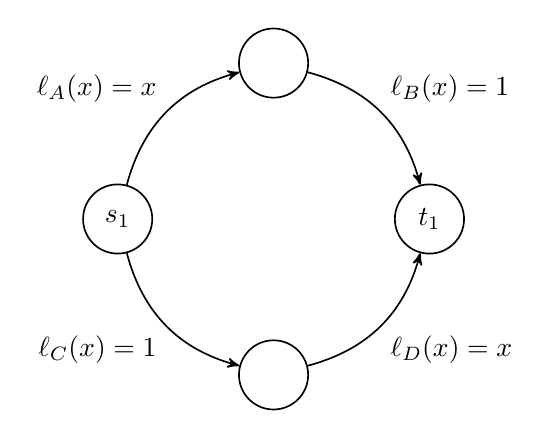
\begin{tikzpicture}[>=stealth',auto,node distance=2.8cm,semithick]
		\tikzstyle{every state}=[draw]

		\node[state] (1) {$s_1$};
		\node[state] (2) [above right of=1] {};
		\node[state] (3) [below right of=1] {};
		\node[state] (4) [below right of=2] {$t_1$};

		\path[->]
		(1) edge [bend left] node {$\ell_A(x)=x$} (2)
			edge [bend right] node [below left] {$\ell_C(x)=1$} (3)
		(2)	edge [bend left] node {$\ell_B(x)=1$} (4)
		(3) edge [bend right] node [below right] {$\ell_D(x)=x$} (4);
	\end{tikzpicture}
\end{center}

We have:
\begin{itemize}
	\item $\ell_A(x) = x$, $\ell_B(x) = 1$, $\ell_C(x) = 1$, $\ell_D(x) = x$
	\item $P = P_1 = \{ (A,B), (C,D) \}$
\end{itemize}

Call $(A,B)$ the ``up'' path, and $(C,D)$ the ``down'' path. Consider the flow
$f$ for $\lambda \in [0,1]$ where $f^\lambda(\text{up}) = \lambda$ and
$f^\lambda(\text{down}) = 1 - \lambda$. We have the following flows on edges:
\begin{equation*}
	\begin{gathered}
		f_A^\lambda = f_B^\lambda = \lambda \\
		f_C^\lambda = f_D^\lambda = 1 - \lambda
	\end{gathered}
\end{equation*}

The latencies of the paths are:
\begin{equation*}
	\begin{gathered}
		L_\text{up}(f^\lambda) = \ell_A(f_A^\lambda) + \ell_B(f_B^\lambda) = \ell_A(\lambda) + \ell_B(\lambda) = \lambda + 1 \\
		L_\text{down}(f^\lambda) = \ell_C(f_C^\lambda) + \ell_D(f_D^\lambda) = \ell_C(1 - \lambda) + \ell_D(1 - \lambda) = 1 + 1 - \lambda = 2 - \lambda
	\end{gathered}
\end{equation*}

The social cost of flow $f^\lambda$ is hence given by:
\begin{equation*}
	\begin{split}
		C(f^\lambda) & = \sum_{p\in P} f^\lambda (p) \cdot L_p(f^\lambda) \\
		& = f^\lambda (\text{up}) \cdot L_\text{up} (f^\lambda) + f^\lambda (\text{down}) \cdot L_\text{down}(f^\lambda) \\
		& = \lambda (1 + \lambda) + (1 - \lambda) (2 - \lambda) \\
		& = 2(\lambda^2 - \lambda + 1) \\
	\end{split}
\end{equation*}

The cost of this flow is minimised by setting $\lambda = 1/2$, which gives a
social cost of $C(f^\frac{1}{2}) = 2(\frac{1}{2}^2 - \frac{1}{2} + 1) = 3/2$.

\subsection{Non-atomic flow games}

So far there has been no game to play -- we could simply compute the
cost-minimising flow and route the traffic as such. However, in selfish routing
we assume that the agents are responsible for routing the traffic, each trying
to minimise his own latency. In this model, there are:

\begin{itemize}
	\item infinitely many player $i \in [0, r]$, each controlling an
		infinitesimal amount of traffic
	\item each player aims to minimise their own latency
\end{itemize}

\textbf{Wardrop's First Principle:} if a route is used, then it is at least as
good as all other routes (otherwise they would simply take another better
route).

\begin{definition}[Wardrop Equilibrium]
	Flow $f$ is a Wardrop Equilibrium (WE) if for every $i \in [k]$, for every
	pair of paths $p, p' \in P_i$, if $f(p) > 0$ then $L_p(f) \le L_{p'}(f)$.
	In other words, whenever there is some flow on some path $p$, then all
	other alternative paths $p'$ have at least the same latency.
\end{definition}

\begin{fact}
	Every flow network has a Wardrop Equilibrium.
\end{fact}

\subsubsection{Example}

\begin{claim}
	The only Wardrop Equilibrium in the previous game is the flow
	$f^\frac{1}{2}$
\end{claim}
\begin{proof}
	First observe that setting $\lambda = 1/2$ is indeed an equilibrium: the
	flow on the ``up'' path is $\lambda + 1$ = 3/2, equal to the flow on the
	``down'' path, $2 - \lambda = 3/2$. Therefore no player has the incentive
	to deviate to the other path, as it would not decrease the latency they
	experience.

	If $\lambda > 1/2$ then the flow on the upper path is non-zero. But
	$L_\text{up}(f^\lambda) = 1 + \lambda > 3/2$, while
	$L_\text{down}(f^\lambda) = 2 - \lambda < 3/2$, so $L_\text{up}(f^\lambda)
	> L_\text{down}(f^\lambda)$, meaning players on the top path would want to
	move to the bottom path.

	If $\lambda < 1/2$ then the flow on the bottom path is non-zero. Then we
	have $L_\text{down}(f^\lambda) > 3/2$ and $L_\text{up}(f^\lambda) < 3/2$,
	so players on the bottom path would want to switch to the top path. Hence
	the flow $f^\frac{1}{2}$ is the only equilibrium.
\end{proof}

\subsubsection{Braess' Paradox}

\begin{center}
	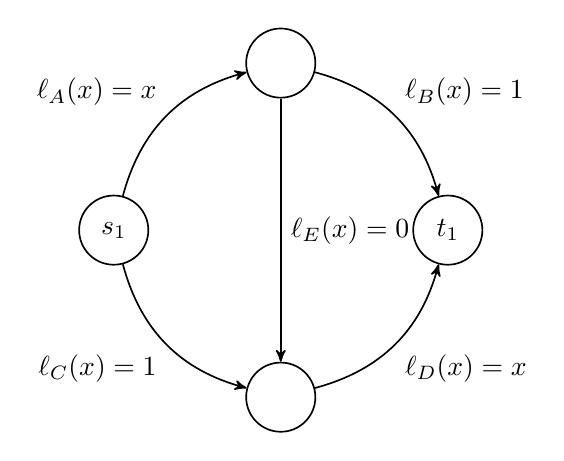
\begin{tikzpicture}[>=stealth',auto,node distance=3cm,semithick]
		\tikzstyle{every state}=[draw]

		\node[state] (1) {$s_1$};
		\node[state] (2) [above right of=1] {};
		\node[state] (3) [below right of=1] {};
		\node[state] (4) [below right of=2] {$t_1$};

		\path[->]
		(1) edge [bend left] node {$\ell_A(x)=x$} (2)
			edge [bend right] node [below left] {$\ell_C(x)=1$} (3)
		(2)	edge [bend left] node {$\ell_B(x)=1$} (4)
		(2)	edge node {$\ell_E(x)=0$} (3)
		(3) edge [bend right] node [below right] {$\ell_D(x)=x$} (4);
	\end{tikzpicture}
\end{center}

We have installed a bridge $E$ that incurs no latency when travelling over it,
that is, $\ell_E(x) = 0$.

We have the paths $P = \{ (A,B), (A,E,D), (C,D) \}$ which we will label ``up'',
``bridge'', and ``down'' respectively. We consider the flow $f^{\conj{\lambda}}
= f^{\lambda_1, \lambda_2, \lambda_3}$ that sends $\lambda_1$ units of flow
through the top path, $\lambda_3$ units through the bottom path, and the
remaining $\lambda_2 = 1 - \lambda_1 - \lambda_3$ units through the bridge
path. The flows are:
\begin{equation*}
	\begin{split}
		f^{\conj{\lambda}}_A & = \lambda_1 + \lambda_2 \\
		f^{\conj{\lambda}}_B & = \lambda_1 \\
		f^{\conj{\lambda}}_C & = \lambda_3 \\
		f^{\conj{\lambda}}_D & = \lambda_2 + \lambda_3 \\
		f^{\conj{\lambda}}_E & = \lambda_2 \\
	\end{split}
\end{equation*}

The latencies are:
\begin{equation*}
	\begin{split}
		L_\text{up}(f^{\conj{\lambda}}) & = \lambda_1 + \lambda_2 + 1 =
		2 - \lambda_3 \\
		L_\text{down}(f^{\conj{\lambda}}) & = 1 + \lambda_2 + \lambda_3 = 2 -
		\lambda_1 \\
		L_\text{bridge}(f^{\conj{\lambda}}) & = \lambda_1 + 2\lambda_2 +
		\lambda_3 = 2 - \lambda_1 - \lambda_3
	\end{split}
\end{equation*}

The minimum social cost is again $3/2$, achieved by flow $f^{\frac{1}{2}, 0,
\frac{1}{2}}$. However, the only Wardrop Equilibrium in this game is the flow
$f^{0,1,0}$, where everyone uses the zero-cost bridge.

\begin{claim}
	The only Wardrop Equilibrium in the game is the flow $f^{0,1,0}$.
\end{claim}
\begin{proof}
	The flow $f^{0,1,0}$ is a Wardrop Equilibrium as $L_\text{up}(f^{0,1,0}) =
	L_\text{down}(f^{0,1,0}) = L_\text{bridge}(f^{0,1,0}) = 2$.

	Now consider the cases where $\lambda_1, \lambda_3 \neq 0$. In either case
	some flow is sent along the ``bridge'' path. If only $\lambda_1 > 0$:
	\begin{itemize}
		\item there is some flow sent along the ``up'' path, and none along the
			``down'' path
		\item $L_\text{up}(f^{\conj{\lambda}}) = 2 > 2 - \lambda_1 =
			L_\text{bridge}(f^{\conj{\lambda}})$
		\item so players have incentive to deviate to taking the ``bridge''
			path
	\end{itemize}

	If only $\lambda_3 > 0$:
	\begin{itemize}
		\item there is some flow sent along the ``down'' path, and none along the
			``up'' path
		\item $L_\text{down}(f^{\conj{\lambda}}) = 2 > 2 - \lambda_3 =
			L_\text{bridge}(f^{\conj{\lambda}})$
		\item so players have incentive to deviate to taking the ``bridge''
			path
	\end{itemize}

	If both $\lambda_1, \lambda_3 > 0$, then all paths are used, and
	$L_\text{bridge}(f^{\conj{\lambda}}) < L_\text{up}(f^{\conj{\lambda}}),
	L_\text{down}(f^{\conj{\lambda}})$.

	Hence whenever $\lambda_1, \lambda_3 > 0$ players always have an incentive
	to deviate to the ``bridge'' path. Therefore the only Wardrop Equilibrium
	is the flow $f^{0,1,0}$.

\end{proof}

\begin{definition}[Price of Anarchy]
	The Price of Anarchy (POA) of a network $G$ is the maximum ratio of
	the cost of the worst possible Wardrop flow and the cost of the optimal
	feasible flow. That is,
	\begin{equation}
		POA(G) = \frac{ \max_{f \text{ is WE}} C(f) }{ \min_{f^* \text{ is
		flow}} C(f^*) }
	\end{equation}
\end{definition}

\begin{fact}
	The Price of Anarchy in Braess' Network is $\frac{2}{3/2} = 4/3$.
\end{fact}

So the Wardrop Equilibrium flow is $1/3$ worse than the optimal in Braess'
Network. This example is interesting as it shows that adding links that seem to
be beneficial may actually degrade performance if the traffic is controlled by
selfish players. We will now cover an even simpler example where the Price of
Anarchy can be made arbitrarily bad.

\subsubsection{Pigou's Network}

\begin{center}
	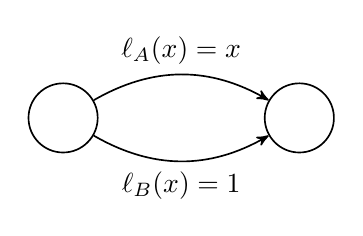
\begin{tikzpicture}[>=stealth',auto,node distance=3cm,semithick]
		\tikzstyle{every state}=[draw]

		\node[state] (1) {};
		\node[state] (2) [right of=1] {};

		\path[->]
		(1) edge [bend left] node {$\ell_A(x)=x$} (2)
			edge [bend right] node [below] {$\ell_B(x)=1$} (2);
	\end{tikzpicture}
\end{center}


The latency functions are $\ell_A(x)=x$, $\ell_B(x)=1$. Consider the flow $f$:
\begin{equation*}
	\begin{split}
		f^\varepsilon : & \, A \mapsto 1 - \varepsilon \\
		& B \mapsto \varepsilon
	\end{split}
\end{equation*}

No matter the value of $\varepsilon$, everyone always wants to take the top
path: sending $\varepsilon$ along edge $B$ incurs a latency of 1, but a latency
of $1-\varepsilon$ along edge $A$. Hence the only Wardrop Equilibrium is $f^0$,
whose social cost is 1. The minimum social cost is achieved by the flow
$f^\frac{1}{2}$, which incurs a social cost of $3/4$. Hence the Price of
Anarchy of the above network is $\frac{1}{3/4} = 4/3$.

\begin{center}
	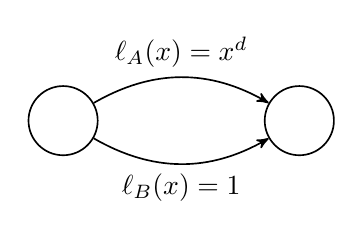
\begin{tikzpicture}[>=stealth',auto,node distance=3cm,semithick]
		\tikzstyle{every state}=[draw]

		\node[state] (1) {};
		\node[state] (2) [right of=1] {};

		\path[->]
		(1) edge [bend left] node {$\ell_A(x)=x^d$} (2)
			edge [bend right] node [below] {$\ell_B(x)=1$} (2);
	\end{tikzpicture}
\end{center}

Now consider the same network with latency functions $\ell_A(x)=x^d$ for $d \in
[0,1]$, and $\ell_B(x)=1$. The flow $f^0$ is still the only Wardrop Equilibrium
with a social cost of $C(f^0) = 1$.

The cost of sending $\varepsilon$ units of flow along $B$ and the remainder
along $A$ is
$$C(f^\varepsilon) = (1-\varepsilon)(1-\varepsilon)^d + 1 \cdot \varepsilon =
\varepsilon + (1-\varepsilon)^{d+1}$$

This is minimised when the derivative is 0:
\begin{equation*}
	\begin{split}
		1 - (d+1)(1-\varepsilon^*)^d & = 0 \\
		\varepsilon^* = 1 - \frac{1}{\sqrt[d]{d+1}}
	\end{split}
\end{equation*}

The cost of this flow is:
\begin{equation*}
	\begin{split}
		C(f^{\varepsilon^*}) & = \varepsilon^* + (1-\varepsilon^*)^{d+1} \\
		& = 1 - \frac{d}{(d+1)\sqrt[d]{d+1}}
	\end{split}
\end{equation*}

As $d \rightarrow \infty$, $C(f^{\varepsilon^*}) \rightarrow 0$. Therefore the
Price of Anarchy ($\frac{\text{stable}}{\text{optimal}}$) is unbounded.

\subsubsection{Pigou Bound}

The latency functions used in Pigou's example are very steep. Can we derive
better bounds on the Price of Anarchy by restricting the kind of
latency functions that are allowed in the network?

\begin{definition}[Pigou Bound]
	Let $\mathcal{C}$ be a set of latency functions. The Pigou Bound
	$\pi(\mathcal{C})$ is defined as follows:
	\begin{equation}
		\pi(\mathcal{C}) = \sup_{\ell \in \mathcal{C}} \sup_{\varepsilon \in
		[0, r]}
		\frac{r \cdot \ell(r)}{\varepsilon \cdot \ell(\varepsilon) +
		(r-\varepsilon) \cdot \ell(r)}
	\end{equation}
\end{definition}

This value is the worst Price of Anarchy possible in a network with two
parallel edges, one with a constant latency function and the other with a
latency function drawn from a set $\mathcal{C}$. The idea is to take the worst
possible latency function $\ell \in \mathcal{C}$ and the worst possible demand
$r$. One of the two edges has constant latency equal to $\ell(r)$, and the
other's latency is given by the latency function $\ell$.

\begin{center}
	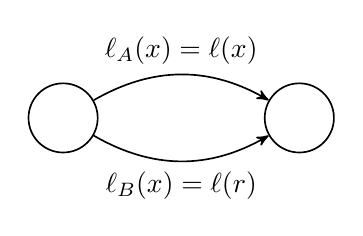
\begin{tikzpicture}[>=stealth',auto,node distance=3cm,semithick]
		\tikzstyle{every state}=[draw]

		\node[state] (1) {};
		\node[state] (2) [right of=1] {};

		\path[->]
		(1) edge [bend left] node {$\ell_A(x)=\ell(x)$} (2)
			edge [bend right] node [below] {$\ell_B(x)=\ell(r)$} (2);
	\end{tikzpicture}
\end{center}

\begin{theorem}
	If a class $\mathcal{C}$ of latency functions contains all constant
	functions, then $POA(\mathcal{C}) \le \pi(\mathcal{C})$.
\end{theorem}

Recall that the Price of Anarchy can be made arbitrarily large, i.e.
$POA(\mathcal{C}) \ge \pi(\mathcal{C})$

\begin{corollary}
	The worst POA in Pigou's Network is equal to the worst POA in all graphs.
\end{corollary}

\begin{theorem}[Variational Inequality Characterisation]
	The flow $f$ is a Wardrop Equilibrium iff for every feasible flow $f^*$ we
	have:
	\begin{equation}
		\sum_{e \in E} f_e \cdot \ell_e(f_e) \le \sum_{e \in E} f^*_e \cdot
		l_e(f_e)
	\end{equation}

	That is, the social cost of $f$ is at most the social cost of $f^*$ in the
	network where each edge has constant latency function $\ell_e(f_e)$.
\end{theorem}
\begin{proof}
	Begin by writing the right hand side of the inequality in terms of paths
	rather than edges and define $H_f(f^*)$ as:
	\begin{equation*}
		\begin{split}
			H_f(f^*) & = \sum_{e \in E} f^*_e \cdot \ell_e(f_e) \\
			& = \sum_{i \in [k]} \sum_{p \in P_i} f^*(p) \cdot L_p(f)
		\end{split}
	\end{equation*}

	Note that the right hand side is equal to $H_f(f^*)$ while the left hand
	side is equal to $H_f(f)$.
\end{proof}


\end{document}
